\documentclass[a4paper]{article}

\def\nterm {Spring}
\def\nyear {2019}
\def\nlecturer {Dr. Barry Ritchie}
\def\ncourse {Classical Particles, Fields, and Matter II}

\RequirePackage{etex}
\makeatletter
\ifx \nauthor\undefined
  \def\nauthor{Daniel Moore}
\else
\fi

\author{Based on lectures by \nlecturer \\\small Notes taken by \nauthor}
\date{\nterm\ \nyear}

\usepackage{alltt}
\usepackage{amsfonts}
\usepackage{amsmath}
\usepackage{amssymb}
\usepackage{amsthm}
\usepackage{booktabs}
\usepackage[makeroom]{cancel}
\usepackage{caption}
\usepackage{enumitem}
\usepackage{fancyhdr}
\usepackage{graphicx}
\usepackage{mathdots}
\usepackage{mathtools}
\usepackage{microtype}
\usepackage{multirow}
\usepackage{pdflscape}
\usepackage{pgfplots}
\usepackage{siunitx}
\usepackage{textcomp}
\usepackage{slashed}
\usepackage{tabularx}
\usepackage{tikz}
\usepackage{tikz-3dplot}
\usepackage{tkz-euclide}
\usepackage{titlesec}
\usepackage[normalem]{ulem}
\usepackage[all]{xy}
\usepackage{imakeidx}

\makeindex[intoc, title=Index]
\indexsetup{othercode={\lhead{\emph{Index}}}}
%\setcounter{secnumdepth}{4}

\titleformat{\paragraph}
{\normalfont\normalsize\bfseries}{\theparagraph}{1em}{}
\titlespacing*{\paragraph}
{0pt}{3.25ex plus 1ex minus .2ex}{1.5ex plus .2ex}

\ifx \nextra \undefined
  \usepackage[pdftex,
    hidelinks,
    pdfauthor={Daniel Moore},
    pdfsubject={\ncourse},
    pdftitle={\ncourse},
  pdfkeywords={\nterm\ \nyear\ \ncourse}]{hyperref}
  \title{\ncourse}
\else
  \usepackage[pdftex,
    hidelinks,
    pdfauthor={Daniel Moore},
    pdfsubject={\ncourse\ (\nextra)},
    pdftitle={\ncourse\ (\nextra)},
  pdfkeywords={\nterm\ \nyear\ \ncourse\ \nextra}]{hyperref}

  \title{\ncourse \\ {\Large \nextra}}
  \renewcommand\printindex{}
\fi

\pgfplotsset{compat=1.12}

\pagestyle{fancyplain}
\ifx \ncoursehead \undefined
\def\ncoursehead{\ncourse}
\fi

\lhead{\emph{\nouppercase{\leftmark}}}
\ifx \nextra \undefined
  \rhead{
    \ifnum\thepage=1
    \else
      \ncoursehead
    \fi}
\else
  \rhead{
    \ifnum\thepage=1
    \else
      \ncoursehead \ (\nextra)
    \fi}
\fi
\usetikzlibrary{arrows.meta}
\usetikzlibrary{decorations.markings}
\usetikzlibrary{decorations.pathmorphing}
\usetikzlibrary{positioning}
\usetikzlibrary{fadings}
\usetikzlibrary{intersections}
\usetikzlibrary{cd}

\newcommand*{\Cdot}{{\raisebox{-0.25ex}{\scalebox{1.5}{$\cdot$}}}}
\newcommand {\pd}[2][ ]{
  \ifx #1 { }
    \frac{\partial}{\partial #2}
  \else
    \frac{\partial^{#1}}{\partial #2^{#1}}
  \fi
}
\newcommand{\pder}[2]{
    \frac{\partial #1}{\partial #2}
}
\newcommand{\dd}[1]{
	\frac{\d}{\d #1}
}
\newcommand{\der}[2]{
	\frac{\d #1}{\d #2}
}
\newcommand{\mbeq}{\overset{!}{=}}
\newcommand{\vhat}[1]{\vec{\hat{#1}}}
\newcommand{\x}{\vhat{x}}
\newcommand{\y}{\vhat{y}}
\newcommand{\z}{\vhat{z}}
\newcommand{\del}{\vec{\nabla}}
\ifx \nhtml \undefined
\else
  \renewcommand\printindex{}
  \DisableLigatures[f]{family = *}
  \let\Contentsline\contentsline
  \renewcommand\contentsline[3]{\Contentsline{#1}{#2}{}}
  \renewcommand{\@dotsep}{10000}
  \newlength\currentparindent
  \setlength\currentparindent\parindent

  \newcommand\@minipagerestore{\setlength{\parindent}{\currentparindent}}
  \usepackage[active,tightpage,pdftex]{preview}
  \renewcommand{\PreviewBorder}{0.1cm}

  \newenvironment{stretchpage}%
  {\begin{preview}\begin{minipage}{\hsize}}%
    {\end{minipage}\end{preview}}
  \AtBeginDocument{\begin{stretchpage}}
  \AtEndDocument{\end{stretchpage}}

  \newcommand{\@@newpage}{\end{stretchpage}\begin{stretchpage}}

  \let\@real@section\section
  \renewcommand{\section}{\@@newpage\@real@section}
  \let\@real@subsection\subsection
  \renewcommand{\subsection}{\@ifstar{\@real@subsection*}{\@@newpage\@real@subsection}}
\fi
\ifx \ntrim \undefined
\else
  \usepackage{geometry}
  \geometry{
    papersize={379pt, 699pt},
    textwidth=345pt,
    textheight=596pt,
    left=17pt,
    top=54pt,
    right=17pt
  }
\fi

\ifx \nisofficial \undefined
\let\@real@maketitle\maketitle
\renewcommand{\maketitle}{\@real@maketitle\begin{center}\begin{minipage}[c]{0.9\textwidth}\centering\footnotesize These notes are not endorsed by the lecturers, and I have modified them (often significantly) after lectures. They are nowhere near accurate representations of what was actually lectured, and in particular, all errors are almost surely mine.\end{minipage}\end{center}}
\else
\fi

% Theorems
\theoremstyle{definition}
\newtheorem*{aim}{Aim}
\newtheorem*{axiom}{Axiom}
\newtheorem*{claim}{Claim}
\newtheorem*{cor}{Corollary}
\newtheorem*{conjecture}{Conjecture}
\newtheorem*{defi}{Definition}
\newtheorem*{eg}{Example}
\newtheorem*{ex}{Exercise}
\newtheorem*{fact}{Fact}
\newtheorem*{law}{Law}
\newtheorem*{lemma}{Lemma}
\newtheorem*{notation}{Notation}
\newtheorem*{prop}{Proposition}
\newtheorem*{question}{Question}
\newtheorem*{problem}{Problem}
\newtheorem*{rrule}{Rule}
\newtheorem*{thm}{Theorem}
\newtheorem*{assumption}{Assumption}

\newtheorem*{remark}{Remark}
\newtheorem*{warning}{Warning}
\newtheorem*{exercise}{Exercise}

\newtheorem{nthm}{Theorem}[section]
\newtheorem{nlemma}[nthm]{Lemma}
\newtheorem{nprop}[nthm]{Proposition}
\newtheorem{ncor}[nthm]{Corollary}


\renewcommand{\labelitemi}{--}
\renewcommand{\labelitemii}{$\circ$}
\renewcommand{\labelenumi}{(\roman{*})}

\let\stdsection\section
\renewcommand\section{\newpage\stdsection}

% Strike through
\def\st{\bgroup \ULdepth=-.55ex \ULset}


%%%%%%%%%%%%%%%%%%%%%%%%%
%%%%% Maths Symbols %%%%%
%%%%%%%%%%%%%%%%%%%%%%%%%

% Matrix groups
\newcommand{\GL}{\mathrm{GL}}
\newcommand{\Or}{\mathrm{O}}
\newcommand{\PGL}{\mathrm{PGL}}
\newcommand{\PSL}{\mathrm{PSL}}
\newcommand{\PSO}{\mathrm{PSO}}
\newcommand{\PSU}{\mathrm{PSU}}
\newcommand{\SL}{\mathrm{SL}}
\newcommand{\SO}{\mathrm{SO}}
\newcommand{\Spin}{\mathrm{Spin}}
\newcommand{\Sp}{\mathrm{Sp}}
\newcommand{\SU}{\mathrm{SU}}
\newcommand{\U}{\mathrm{U}}
\newcommand{\Mat}{\mathrm{Mat}}

% Matrix algebras
\newcommand{\gl}{\mathfrak{gl}}
\newcommand{\ort}{\mathfrak{o}}
\newcommand{\so}{\mathfrak{so}}
\newcommand{\su}{\mathfrak{su}}
\newcommand{\uu}{\mathfrak{u}}
\renewcommand{\sl}{\mathfrak{sl}}

% Special sets
\newcommand{\C}{\mathbb{C}}
\newcommand{\CP}{\mathbb{CP}}
\newcommand{\GG}{\mathbb{G}}
\newcommand{\N}{\mathbb{N}}
\newcommand{\Q}{\mathbb{Q}}
\newcommand{\R}{\mathbb{R}}
\newcommand{\RP}{\mathbb{RP}}
\newcommand{\T}{\mathbb{T}}
\newcommand{\Z}{\mathbb{Z}}
\renewcommand{\H}{\mathbb{H}}

% Brackets
\newcommand{\abs}[1]{\left\lvert #1\right\rvert}
\newcommand{\bket}[1]{\left\lvert #1\right\rangle}
\newcommand{\brak}[1]{\left\langle #1 \right\rvert}
\newcommand{\braket}[2]{\left\langle #1\middle\vert #2 \right\rangle}
\newcommand{\bra}{\langle}
\newcommand{\ket}{\rangle}
\newcommand{\norm}[1]{\left\lVert #1\right\rVert}
\newcommand{\normalorder}[1]{\mathop{:}\nolimits\!#1\!\mathop{:}\nolimits}
\newcommand{\tv}[1]{|#1|}
\renewcommand{\vec}[1]{\boldsymbol{\mathbf{#1}}}

% not-math
\newcommand{\bolds}[1]{{\bfseries #1}}
\newcommand{\cat}[1]{\mathsf{#1}}
\newcommand{\ph}{\,\cdot\,}
\newcommand{\term}[1]{\emph{#1}\index{#1}}
\newcommand{\phantomeq}{\hphantom{{}={}}}
% Probability
\DeclareMathOperator{\Bernoulli}{Bernoulli}
\DeclareMathOperator{\betaD}{beta}
\DeclareMathOperator{\bias}{bias}
\DeclareMathOperator{\binomial}{binomial}
\DeclareMathOperator{\corr}{corr}
\DeclareMathOperator{\cov}{cov}
\DeclareMathOperator{\gammaD}{gamma}
\DeclareMathOperator{\mse}{mse}
\DeclareMathOperator{\multinomial}{multinomial}
\DeclareMathOperator{\Poisson}{Poisson}
\DeclareMathOperator{\var}{var}
\newcommand{\E}{\mathbb{E}}
\newcommand{\Prob}{\mathbb{P}}

% Algebra
\DeclareMathOperator{\adj}{adj}
\DeclareMathOperator{\Ann}{Ann}
\DeclareMathOperator{\Aut}{Aut}
\DeclareMathOperator{\Char}{char}
\DeclareMathOperator{\disc}{disc}
\DeclareMathOperator{\dom}{dom}
\DeclareMathOperator{\fix}{fix}
\DeclareMathOperator{\Hom}{Hom}
\DeclareMathOperator{\id}{id}
\DeclareMathOperator{\image}{image}
\DeclareMathOperator{\im}{im}
\DeclareMathOperator{\re}{re}
\DeclareMathOperator{\tr}{tr}
\DeclareMathOperator{\Tr}{Tr}
\newcommand{\Bilin}{\mathrm{Bilin}}
\newcommand{\Frob}{\mathrm{Frob}}

% Others
\newcommand\ad{\mathrm{ad}}
\newcommand\Art{\mathrm{Art}}
\newcommand{\B}{\mathcal{B}}
\newcommand{\cU}{\mathcal{U}}
\newcommand{\Der}{\mathrm{Der}}
\newcommand{\D}{\mathrm{D}}
\newcommand{\dR}{\mathrm{dR}}
\newcommand{\exterior}{\mathchoice{{\textstyle\bigwedge}}{{\bigwedge}}{{\textstyle\wedge}}{{\scriptstyle\wedge}}}
\newcommand{\F}{\mathbb{F}}
\newcommand{\G}{\mathcal{G}}
\newcommand{\Gr}{\mathrm{Gr}}
\newcommand{\haut}{\mathrm{ht}}
\newcommand{\Hol}{\mathrm{Hol}}
\newcommand{\hol}{\mathfrak{hol}}
\newcommand{\I}{\mathbb{I}}
\newcommand{\Id}{\mathrm{Id}}
\newcommand{\Lp}{\mathcal{L}}
\newcommand{\lie}[1]{\mathfrak{#1}}
\newcommand{\op}{\mathrm{op}}
\newcommand{\Oc}{\mathcal{O}}
\newcommand{\pr}{\mathrm{pr}}
\newcommand{\Ps}{\mathcal{P}}
\newcommand{\pt}{\mathrm{pt}}
\newcommand{\qeq}{\mathrel{``{=}"}}
\newcommand{\Rs}{\mathcal{R}}
\newcommand{\Vect}{\mathrm{Vect}}
\newcommand{\wsto}{\stackrel{\mathrm{w}^*}{\to}}
\newcommand{\wt}{\mathrm{wt}}
\newcommand{\wto}{\stackrel{\mathrm{w}}{\to}}
\renewcommand{\d}{\mathrm{d}}
\renewcommand{\P}{\mathbb{P}}
%\renewcommand{\F}{\mathcal{F}}


\let\Im\relax
\let\Re\relax

\DeclareMathOperator{\area}{area}
\DeclareMathOperator{\card}{card}
\DeclareMathOperator{\ccl}{ccl}
\DeclareMathOperator{\ch}{ch}
\DeclareMathOperator{\cl}{cl}
\DeclareMathOperator{\cls}{\overline{\mathrm{span}}}
\DeclareMathOperator{\coker}{coker}
\DeclareMathOperator{\conv}{conv}
\DeclareMathOperator{\cosec}{cosec}
\DeclareMathOperator{\cosech}{cosech}
\DeclareMathOperator{\covol}{covol}
\DeclareMathOperator{\diag}{diag}
\DeclareMathOperator{\diam}{diam}
\DeclareMathOperator{\Diff}{Diff}
\DeclareMathOperator{\End}{End}
\DeclareMathOperator{\energy}{energy}
\DeclareMathOperator{\erfc}{erfc}
\DeclareMathOperator{\erf}{erf}
\DeclareMathOperator*{\esssup}{ess\,sup}
\DeclareMathOperator{\ev}{ev}
\DeclareMathOperator{\Ext}{Ext}
\DeclareMathOperator{\fst}{fst}
\DeclareMathOperator{\Fit}{Fit}
\DeclareMathOperator{\Frac}{Frac}
\DeclareMathOperator{\Gal}{Gal}
\DeclareMathOperator{\gr}{gr}
\DeclareMathOperator{\hcf}{hcf}
\DeclareMathOperator{\Im}{Im}
\DeclareMathOperator{\Ind}{Ind}
\DeclareMathOperator{\Int}{Int}
\DeclareMathOperator{\Isom}{Isom}
\DeclareMathOperator{\lcm}{lcm}
\DeclareMathOperator{\length}{length}
\DeclareMathOperator{\Lie}{Lie}
\DeclareMathOperator{\like}{like}
\DeclareMathOperator{\Lk}{Lk}
\DeclareMathOperator{\Maps}{Maps}
\DeclareMathOperator{\orb}{orb}
\DeclareMathOperator{\ord}{ord}
\DeclareMathOperator{\otp}{otp}
\DeclareMathOperator{\poly}{poly}
\DeclareMathOperator{\rank}{rank}
\DeclareMathOperator{\rel}{rel}
\DeclareMathOperator{\Rad}{Rad}
\DeclareMathOperator{\Re}{Re}
\DeclareMathOperator*{\res}{res}
\DeclareMathOperator{\Res}{Res}
\DeclareMathOperator{\Ric}{Ric}
\DeclareMathOperator{\rk}{rk}
\DeclareMathOperator{\Rees}{Rees}
\DeclareMathOperator{\Root}{Root}
\DeclareMathOperator{\sech}{sech}
\DeclareMathOperator{\sgn}{sgn}
\DeclareMathOperator{\snd}{snd}
\DeclareMathOperator{\Spec}{Spec}
\DeclareMathOperator{\spn}{span}
\DeclareMathOperator{\stab}{stab}
\DeclareMathOperator{\St}{St}
\DeclareMathOperator{\supp}{supp}
\DeclareMathOperator{\Syl}{Syl}
\DeclareMathOperator{\Sym}{Sym}
\DeclareMathOperator{\vol}{vol}

\pgfarrowsdeclarecombine{twolatex'}{twolatex'}{latex'}{latex'}{latex'}{latex'}
\tikzset{->/.style = {decoration={markings,
                                  mark=at position 1 with {\arrow[scale=2]{latex'}}},
                      postaction={decorate}}}
\tikzset{<-/.style = {decoration={markings,
                                  mark=at position 0 with {\arrowreversed[scale=2]{latex'}}},
                      postaction={decorate}}}
\tikzset{<->/.style = {decoration={markings,
                                   mark=at position 0 with {\arrowreversed[scale=2]{latex'}},
                                   mark=at position 1 with {\arrow[scale=2]{latex'}}},
                       postaction={decorate}}}
\tikzset{->-/.style = {decoration={markings,
                                   mark=at position #1 with {\arrow[scale=2]{latex'}}},
                       postaction={decorate}}}
\tikzset{-<-/.style = {decoration={markings,
                                   mark=at position #1 with {\arrowreversed[scale=2]{latex'}}},
                       postaction={decorate}}}
\tikzset{->>/.style = {decoration={markings,
                                  mark=at position 1 with {\arrow[scale=2]{latex'}}},
                      postaction={decorate}}}
\tikzset{<<-/.style = {decoration={markings,
                                  mark=at position 0 with {\arrowreversed[scale=2]{twolatex'}}},
                      postaction={decorate}}}
\tikzset{<<->>/.style = {decoration={markings,
                                   mark=at position 0 with {\arrowreversed[scale=2]{twolatex'}},
                                   mark=at position 1 with {\arrow[scale=2]{twolatex'}}},
                       postaction={decorate}}}
\tikzset{->>-/.style = {decoration={markings,
                                   mark=at position #1 with {\arrow[scale=2]{twolatex'}}},
                       postaction={decorate}}}
\tikzset{-<<-/.style = {decoration={markings,
                                   mark=at position #1 with {\arrowreversed[scale=2]{twolatex'}}},
                       postaction={decorate}}}

\tikzset{circ/.style = {fill, circle, inner sep = 0, minimum size = 3}}
\tikzset{scirc/.style = {fill, circle, inner sep = 0, minimum size = 1.5}}
\tikzset{mstate/.style={circle, draw, blue, text=black, minimum width=0.7cm}}

\tikzset{eqpic/.style={baseline={([yshift=-.5ex]current bounding box.center)}}}
\tikzset{commutative diagrams/.cd,cdmap/.style={/tikz/column 1/.append style={anchor=base east},/tikz/column 2/.append style={anchor=base west},row sep=tiny}}

\definecolor{mblue}{rgb}{0.2, 0.3, 0.8}
\definecolor{morange}{rgb}{1, 0.5, 0}
\definecolor{mgreen}{rgb}{0.1, 0.4, 0.2}
\definecolor{mred}{rgb}{0.5, 0, 0}

\def\drawcirculararc(#1,#2)(#3,#4)(#5,#6){%
    \pgfmathsetmacro\cA{(#1*#1+#2*#2-#3*#3-#4*#4)/2}%
    \pgfmathsetmacro\cB{(#1*#1+#2*#2-#5*#5-#6*#6)/2}%
    \pgfmathsetmacro\cy{(\cB*(#1-#3)-\cA*(#1-#5))/%
                        ((#2-#6)*(#1-#3)-(#2-#4)*(#1-#5))}%
    \pgfmathsetmacro\cx{(\cA-\cy*(#2-#4))/(#1-#3)}%
    \pgfmathsetmacro\cr{sqrt((#1-\cx)*(#1-\cx)+(#2-\cy)*(#2-\cy))}%
    \pgfmathsetmacro\cA{atan2(#2-\cy,#1-\cx)}%
    \pgfmathsetmacro\cB{atan2(#6-\cy,#5-\cx)}%
    \pgfmathparse{\cB<\cA}%
    \ifnum\pgfmathresult=1
        \pgfmathsetmacro\cB{\cB+360}%
    \fi
    \draw (#1,#2) arc (\cA:\cB:\cr);%
}
\newcommand\getCoord[3]{\newdimen{#1}\newdimen{#2}\pgfextractx{#1}{\pgfpointanchor{#3}{center}}\pgfextracty{#2}{\pgfpointanchor{#3}{center}}}

\newcommand\qedshift{\vspace{-17pt}}
\newcommand\fakeqed{\pushQED{\qed}\qedhere}

\def\Xint#1{\mathchoice
   {\XXint\displaystyle\textstyle{#1}}%
   {\XXint\textstyle\scriptstyle{#1}}%
   {\XXint\scriptstyle\scriptscriptstyle{#1}}%
   {\XXint\scriptscriptstyle\scriptscriptstyle{#1}}%
   \!\int}
\def\XXint#1#2#3{{\setbox0=\hbox{$#1{#2#3}{\int}$}
     \vcenter{\hbox{$#2#3$}}\kern-.5\wd0}}
\def\ddashint{\Xint=}
\def\dashint{\Xint-}

\newcommand\separator{{\centering\rule{2cm}{0.2pt}\vspace{2pt}\par}}

\newenvironment{own}{\color{gray!70!black}}{}

\newcommand\makecenter[1]{\raisebox{-0.5\height}{#1}}

\mathchardef\mdash="2D

\newenvironment{significant}{\begin{center}\begin{minipage}{0.9\textwidth}\centering\em}{\end{minipage}\end{center}}
\DeclareRobustCommand{\rvdots}{%
  \vbox{
    \baselineskip4\p@\lineskiplimit\z@
    \kern-\p@
    \hbox{.}\hbox{.}\hbox{.}
  }}
\DeclareRobustCommand\tph[3]{{\texorpdfstring{#1}{#2}}}
\makeatother


\begin{document}
\maketitle

\tableofcontents

\section{Introduction}
\section{Electrostatics}
\subsection{The Electric Field}
\subsubsection{Definitions and Properties}
\begin{defi}[Electrostatics]
	An \emph{electrostatic} situation is one in which the source charges
	are all stationary, and the electric fields are never changing.
\end{defi}
\begin{defi}[Field point]
	A \emph{field point} is the location of any point in a field (in our
	case, in the electric field). It will be denoted with
	$\vec{r}$ (without a prime).
\end{defi}
\begin{defi}[Source point]
	A \emph{source point} is the location of a charge source. If there
	a number of charges, the principle of linear superposition can usually
	be applied. It will be denoted with $\vec{r}'$ (with a prime).
\end{defi}
We have found experimentally that the force exerted by some point charge, $q$,
at location $\vec{r}'$,
on some test charge, $Q$, at location $\vec{r}$, is given by
\textbf{Coulomb's law}:
\[ \vec{F} = \frac{1}{4\pi\epsilon_0}\frac{qQ}{\rcurs^2} \hrcurs \]
Where $\brcurs = \vec{r}-\vec{r}'$.

We also say that the electrostatic force on a small test charge is given by
\[ \vec{F} = Q\vec{E}(\vec{r}) \]

Since the test charge is small enough that it doesn't distort  the electric
field, we can combine these two things to say that the electric field produced
at a point $\vec{r}$ by a test charge $q$ at point $\vec{r}'$ is given by:
\[ \vec{E} = \frac{1}{4\pi\epsilon_0}\frac{1}{\rcurs^2}\hrcurs \]
If there are a number of source point charges, we can use the principle of
linear superposition and add each of the source points, and add each of the
$q_i$ values, and treat the system as if it is coming from a single charge
of strength $\sum q_i$ at the point $\sum \vec{r'_i}$. We can write this as:
\[ \vec{E}(\vec{r}) = \frac{1}{4\pi\epsilon_0} \sum_{i=1}^{N} \frac{q_i}
{\rcurs_i^2} \hrcurs_i \]
Where $\brcurs_i = \vec{r}-\vec{r}_i$. Note that the field point doesn't
change.

If there is a continuous distribution of charge, we can integrate instead of
summing:
\[ \vec{E}(\vec{r}) = \frac{1}{4\pi\epsilon_0}\int\frac{\d q}{\rcurs^2}
\hrcurs \]
There are three possibilities in this case, depending on if our problem is in
one, two, or three dimensions (ie. a line, a surface, or a volume):
\begin{align*}
	\d q = \lambda\d\ell' && \d q = \sigma\d a' && \d q = \rho\d\tau'
\end{align*}

\subsubsection{Vector Integral Theorems: Divergence}
\begin{defi}[Divergence]
	The divergence of the vector $\vec{G}$ gives the net source density of
	the field at the point in space where it's evaluated.
\end{defi}
Generally, the divergence should look something like:
\[ \del\cdot\vec{G} = \frac{\text{Number of Sources} - \text{Number of Sinks}}
{\text{Volume as it approaches } 0} \cdot \text{Proportionality constant} \]
For an electric field specifically, we would expect
\[ \del\cdot\vec{E} = \frac{\text{Net electric charge}}
{\text{Volume as it appraches } 0} \cdot\text{Constant} \]
We already know that for a continuous charge distribution in a volume,
\[ \vec{E}(\vec{r}) = \frac{1}{4\pi\epsilon_0}\int\frac{\rho(\vec{r}')\d\tau'}
{\rcurs^2}\hrcurs \]
Thus, we can say explicitly,
\begin{align*}
\del\cdot\vec{E}(\vec{r}) &= \frac{1}{4\pi\epsilon_0}\int\rho(\vec{r}')\d\tau'
\del\cdot\left(\frac{\hrcurs}{\rcurs^2}\right)\\
\intertext{We know from 302 that we can simplify the far-right side
using the identity}
\del\cdot\left(\frac{\hrcurs}{\rcurs}\right) &= 4\pi\delta^3(\rcurs)
\intertext{So we can say that}
\del\cdot\vec{E}(\vec{r}) &= \frac{1}{4\pi\epsilon_0}\int\rho(\vec{r}')\d\tau'
\cdot 4\pi\delta^3(\brcurs)\\
&= \frac{1}{4\pi\epsilon_0}\int\rho(\vec{r}')\d\tau'
\cdot 4\pi\delta^3(\vec{r}-\vec{r}')\\
\del\cdot\vec{E}(\vec{r}) &= \frac{\rho(\vec{r})}{\epsilon_0}
\end{align*}
This result is the first of two things that we call ``Gauss's Law.'' To
differentiate the two, we call this the ``differential form.''
\begin{defi}[The divergene theorem of Gauss]
\begin{align*}
	\iiint_V\del\cdot\vec{E}\d\tau = \iint_C\vec{E}\d\vec{a}
\end{align*}
\end{defi}
We know that we can simplify this using the differential form of Gauss's
law, and from there we can solve the left-hand side of this integral:
\begin{align*}
	\iiint_V \frac{\rho(\vec{r})}{\epsilon_0}\d\tau &=
	\frac{1}{\epsilon_0}\iiint_V\rho(\vec{r})\d\tau\\
	&= \frac{Q_{encl}}{\epsilon_0}
\end{align*}
Then, using the divergence theorem, we can conclude that
\[
	\iint_C \vec{E}\cdot\d\vec{a} = \frac{Q_{encl}}{\epsilon_0}
\]
This is the other thing we call ``Gauss's Law,'' and this one we call
the ``integral form.''

The integral form of Gauss's law is always true, but only sometimes useful in
problems. Usually, it is only useful if you can define a ``Gaussian surface''
$S$, where:
\begin{itemize}
	\item The electric firld is everywhere normal to the surface (and
	therefore to the infinitesimal surface piece $\d\vec{a}$)
	\item The electric field is constant over the surface
	\item The charge density $\rho(\vec{r})$ is defined and finite
	everywhere in the volume $V$ contained in $S$
\end{itemize}
However, if these are all satisfied, it is \emph{very} useful, as the
left-hand side of the equation can be simplifed to
$\lvert\vec{E}\rvert A = EA$, where $A$ is the surface area of the
Gaussian surface, meaning the full equation can be simplified to
\[ E = \frac{Q_{encl}}{\epsilon_0 A} \]

\begin{eg}
A long cylinder carries a charge density thatr is perpendicular to the distance
from its axis, $\rho = ks$. Find the electric field inside the cylinder.\\
\textbf{Solution.}
With cylindrical symmetry, we can choose a cylindrical Gaussian surface of
length $\ell$ and radius $s$. We can ignore the contributions of the end-caps
of the surface, since the electric field will be parallel at those points, not
normal. By symmetry, $\vec{E}$ is parallel to $\d\vec{a}$, so the left-hand
side of the equation becomes $EA = 2\pi s\ell$.

The charge enclosed is
\[
Q_{encl} = \int\rho\d\tau'=\iiint_Vks'\d s'\cdot s'\d\phi'\cdot\d z'
	= 2\pi k\ell\int_0^s s'^2\d s' = \frac{2}{3}\pi k\ell s^3
\]
Thus,
\begin{align*}
	EA &= \frac{Q_{encl}}{\epsilon_0}\\
	E\cdot 2\pi s\ell &= \frac{2}{3\epsilon_0}\pi k\ell s^3\\
	E &= \frac{k}{3\epsilon_0}s^2\\
	\vec{E} &= \frac{k}{3\epsilon_0}s^2\hat{\vec{s}}\\
\end{align*}
\end{eg}

\subsubsection{Vector Integral Theorems: Curl}
Suppose we have a point charge $Q$ at the origin of our coordinate system (so
that $\vec{r}' = \vec{0}$).
Then, $\rcurs = \vec{r}$ and $\hrcurs = \hat{\vec{r}}$.
In spherical coordinates,
\begin{align*}
	\vec{E}\cdot\d\vec{\ell} &= \left(\frac{Q}{4\pi\epsilon_0}
	\frac{\vhat{r}}{r^2}\right)\cdot
	(\d r\vhat{r}+r\d\theta\vhat{\theta}+r\sin(\phi)\d\phi\vhat\phi)\\
	&= \frac{Q}{4\pi\epsilon_0}\frac{\d r}{r^2}
\end{align*}
Thus, the integral over some path $C$ would be
\begin{align*}
	\int_C\vec{E}\cdot\d\vec{\ell} &=
		\int_C \frac{Q}{4\pi\epsilon_0}\frac{\d r}{r^2}\\
	&= -\frac{Q}{4\pi\epsilon_0}\left(\frac{1}{r_2}-\frac{1}{r_1}\right)
\end{align*}
We can see clearly that any closed path (ie. one where $r_2=r_1$) would give us
\[ 
	\int_C\vec{E}\cdot\d\vec{\ell} = 0
\]
We could generalize this. Since the electric field obeys the principle of
superposition, this is true for a closed path over any number of source charges
some distance apart.

\begin{defi}[The curl theorem of Stokes]
	\[ \oint_C \vec{E}\cdot\d\vec{\ell} = \iint_S (\del\times\vec{E})
	\cdot\d\vec{a} \]
\end{defi}

Shockingly enough, the left-hand side of that theorem looks a lot like what
we found for a closed path over an electric field. Since we found that that
must equal zero, that means the right-hand side must also always equal zero for
a closed path, and the only way to guarantee that is to say that for any
closed path,
\[ \del\times\vec{E}=0\]
in electrostatics.

Since we know that the electrostatic force is $\vec{F} = Q\vec{E}$, then for
any electrostatic force,
\begin{align*}
	W &= \oint \vec{F}\cdot\d\vec{\ell}\\
	  &= Q\oint\vec{E}\cdot\d\vec{\ell}\\
	  &= 0
\end{align*}
This means that the electrostatic force $\vec{F}$ \emph{must} be a conservative
force. From 310, we know that this means it must be path-independent, and there
must be some potential energy function such that $\vec{F} = -\del U$.

\subsubsection{The Helmholtz Theorem}
\begin{thm}[The Helmholtz theorem]
	For some vector $\vec{G}(\vec{r})$, if
	\begin{itemize}
		\item The divergence $D(\vec{r})$ and the curl 
			$\vec{C}(\vec{r})$ for $\vec{G}(\vec{r})$ are
			specified, and
		\item Both $D(\vec{r})$ and $\vec{C}(\vec{r})$ go to zero
			faster than $r^{-2}$ as $\vec{r}$ approaches infinity,
			and
		\item $\vec{G}(\vec{r})$ goes to zero as $\vec{r}$ goes to
			infinity,
	\end{itemize}
	then the vector field $\vec{G}(\vec{r})$ is given uniquely by the
	expression 
	\[ \vec{G}(\vec{r}) = -\del V(\vec{r}) + \del\times\vec{W}(\vec{r})\]
	where
	\begin{align*}
		V(\vec{r}) = \frac{1}{4\pi}\int\frac{D(\vec{r}')}{\rcurs}
			\d\tau'
		&&
		\vec{W}(\vec{r}) = \frac{1}{4\pi}\int\frac{\vec{C}(\vec{r})}
			{\rcurs}\d\tau'
	\end{align*}
\end{thm}
We can use this theorem to find some interesting things about the electric
field. If these are satisfied for some $\vec{E}(\vec{r})$ (which they
generally are), then we can guarantee a unique form for the electric
field equation. But based on what we now know about the properties of the
divergence and curl of the electric field, we can simplify it a little bit.
For example, we know that over a closed path, the curl of an electric field
is zero, so we know that $\vec{W}(\vec{r}) = 0$, meaning we can write
the electric field uniquely as
\[ \vec{E}(\vec{r}) = -\del V(\vec{r}) \]
where
\begin{align*}
	V(\vec{r}) &= \frac{1}{4\pi}\int\frac{D(\vec{r}')}{\rcurs}\d\tau'\\
		   &= \frac{1}{4\pi\epsilon_0}\int\frac{\rho(\vec{r}')}
			{\rcurs}\d\tau'
\end{align*}
This scalar function $V(\vec{r})$ is called the \textbf{electric potential}
(not to be confused with potential energy).

\subsection{The Electric Potential}
\subsubsection{Definition and Properties}
Using the relationship $\vec{E}(\vec{r})=-\del V(\vec{r})$ we can further
define
\[ V(\vec{r}) = -\int_{\vec{r}_{ref}}^{\vec{r}} \vec{E}\cdot\d\vec{\ell} \]
to be the \textbf{electric potential at point} $\vec{r}$. Typically, we will
pick $\vec{r}_{ref}$ to be $\infty$ as long as the charge distribution is
finite.

\begin{prop}
	The potential differents between points $\vec{r}_a$ and $\vec{r}_b$ is
	\[ -\int_{\vec{r}_a}^{\vec{r}_b} \vec{E}\cdot\d\vec{\ell} \]
\end{prop}
\begin{proof}
\begin{align*}
	V(\vec{r}_b) - V(\vec{r}_a)
	&= -\int_{\vec{r}_{ref}}^{\vec{r}_b} \vec{E}\cdot\d\vec{\ell} -
	\left(-\int_{\vec{r}_{ref}}^{\vec{r}_a}\vec{E}\cdot\d\vec{\ell}\right)\\
	&= -\int_{\vec{r}_{ref}}^{\vec{r}_b} \vec{E}\cdot\d\vec{\ell}
	-\int_{\vec{r}_{a}}^{\vec{r}_{ref}} \vec{E}\cdot\d\vec{\ell}\\
	\Delta V &= -\int_{\vec{r}_a}^{\vec{r}_b}\vec{E}\cdot\d\vec{\ell}
\end{align*}
\end{proof}
Note here that the reference point is irrelevant!
Generally, for a finite distribution, we can expect $\vec{E}\to0$ as
$\vec{r}\to\infty$, so it makes sense to choose $\vec{r}_{ref}=\infty$.

\begin{eg}
	A hollow sphere of radius $R$ is centered on the origin, and has a
	charge $q$ distributed evenly on its surface. What is the electric
	potential at a point $P$ where $P$ is
	\begin{enumerate}
		\item Outside the sphere
		\item Inside the sphere
	\end{enumerate}
	\textbf{Solution.}
	By the integral form of Gauss's law, using a Gaussian surface inside
	and outside the sphere, the electric field is given by
	\[
		\vec{E} = \begin{cases}
			\frac{q}{4\pi\epsilon_0}\frac{\vhat{r}}{r^2}, &
				r > R\\
			0, &
				r < R
	\]
	\begin{enumerate}
		\item The electric field outside the sphere is
		\[ \vec{E} = \frac{q}{4\pi\epsilon_0}\frac{\vhat{r}}{r^2} \]
		Meaning
		\begin{align*}
			V &= -\int_\infty^r \frac{q}{4\pi\epsilon_0}
			\frac{\vhat{r}}{r^2}\cdot \d\vec{\ell}\\
			&= -\int_\infty^r \frac{q}{4\pi\epsilon_0}
			\frac{\d r'}{r'^2}\\
			&= \left.\frac{q}{4\pi\epsilon_0 r'}\right|_\infty^r\\
			V(r) &= \frac{q}{4\pi\epsilon_0 r}
		\end{align*}
	\end{enumerate}
\end{eg}

\begin{eg}
	What is the electric potential $V$ for an infinite uniform plane of
	charge density $\sigma$ lying in the $x-y$ plane for points $P$ where
	$z > 0$?\\
	\textbf{Solution.}
	Using Gauss's law, we know the electric field is given by
	\[ \vec{E} = \frac{\sigma}{2\epsilon_0}\z \]
	We can do the same thing as before, using $\vec{r}_{ref} = \infty$:
	\begin{align*}
		V(\vec{r}) &= -\int_\infty^{\vec{r}}\frac{\sigma}{2\epsilon_0}
		\z\cdot\d\vec{\ell}\\
		V(z) &= -\int_\infty^{z}\frac{\sigma}{2\epsilon_0}\d z'\\
		     &= -\frac{\sigma}{2\epsilon_0}z + \infty\\
		     &= \infty
	\end{align*}
	This obviously doesn't work! This doesn't satisfy the Helmholtz
	conditions, since $\vec{E}$ doesn't disappear as $r\to\infty$.
	Instead, we should choose a reference point on or near the charge
	distribution. Let's pick $z=0$:
	\begin{align*}
		V(z) &= -\int_0^{z}\frac{\sigma}{2\epsilon_0}\d z'\\
		     &= -\frac{\sigma}{2\epsilon_0} z
	\end{align*}
\end{eg}

\subsubsection{The Equations of Poisson and Laplace}
We know the differential forms of Maxwell's equations for electrostatics:
\begin{align*}
	\del\cdot\vec{E} &= \frac{\rho}{\epsilon_0}\\
	\del\times\vec{E} &= 0
\end{align*}
We also know the definition of the potential from the Helmholtz theorem in the
previous subsubsection.

Since $\vec{E}=-\del V$, we can operate on $-\del V$ to find out things about
$\vec{E}$ that might otherise be difficult to determine. First, we can
prove the trivial fact that
\[
	-\del\times\del V = 0
\]
We can find more useful things, though:
\begin{align*}
	\del\cdot(-\del V) = -\nabla^2 V=-\left(\pder{^2V}{x^2} +
		\pder{^2V}{y^2} + \pder{^2V}{z^2}\right)
\end{align*}
Since we know that
\[ \del\cdot\vec{E} = \frac{\rho}{\epsilon_0}\]
we can conclude that
\[\nabla^2V = -\frac{\rho}{\epsilon_0} \]
This is super important! This is a second-order differential equation of a
scalar function $V$. There are two potential situations that this equation
describes:
\begin{enumerate}
	\item $\rho = 0$, ie. there is no charge in the region of interest.
		In this case, this becomes Laplace's equation,
		\[ \nabla^2 V = 0 \]
	\item $\rho \neq 0$, ie. there is some charge in the region of
		interest. In this case, this becomes Poisson's equation,
		\[ \nabla^2 V = -\frac{\rho}{\epsilon_0} \]
\end{enumerate}

\subsection{Work and Energy in Electrostatics}
\subsubsection{Relationship Between Work and the Electric Potential}
The increment of work we do moving against an electric force $\vec{F}$ over a
small displacement $\d\vec{\ell}$ is given by
\[ \d W = -\vec{F}\cdot\d\vec{\ell} = -(Q\vec{E})\cdot\d\vec{\ell} \]
For electrostatics, the total work needed to move a charge from
$\vec{r}_a$ to $\vec{r}_b$ in such an electric field is given by
\[ W = -\int_{\vec{r}_a}^{\vec{r}_b}\vec{F}\cdot\d\vec{\ell}
= -Q\int_{\vec{r}_a}^{\vec{r}_b}\vec{E}\cdot\d\vec{\ell} 
= Q[V(\vec{r}_b) - V(\vec{r}_a)] \]
Note that because the electrostati force is conservative, the work
is path-independent. The work per unit charge can be found easily from this
as
\[ \frac{W}{Q} = V(\vec{r}_b)-V(\vec{r}_a) \]

If we have a finite charge distribution, then using $\vec{r}_{ref} = \infty$,
the work needed to the charge from $\vec{r}_{ref}$ to $\vec{r}_a$ is given by
\[ W = Q[V(\vec{r})-V(\infty)] = QV(\vec{r}) \]

\subsubsection{Energies Associated with Assemblies of Electric Charge}
\begin{eg}
How much work does it take to assemble a distribution of 3 charges $q_1$,
$q_2$, and $q_3$, in that order, with no other electric charges nearby?\\
\textbf{Solution.}
There is no electric field/force to bring $q_1$, so $W_1 = 0$.
For $q_2$:
\begin{align*}
	W_2 &= q_2 V_1(q_1)\\
	    &= q_2\frac{1}{4\pi\epsilon_0}\frac{q_1}{\rcurs_{12}}\\
	    &= \frac{1}{4\pi\epsilon_0}\frac{q_1q_2}{\rcurs_{12}}
\end{align*}
For $q_3$:
\begin{align*}
	W_3 &= q_3V_1(q_1) + q_3V_2(q_2)\\
	    &= q_3\left(\frac{1}{4\pi\epsilon_0}\frac{q_1}{\rcurs_{13}} +
		\frac{1}{4\pi\epsilon_0}\frac{q_2}{\rcurs_{23}}\right)\\
	    &= \frac{1}{4\pi\epsilon_0}\frac{q_1q_3}{\rcurs_{13}} +
		\frac{1}{4\pi\epsilon_0}\frac{q_2q_3}{\rcurs_{23}}
\end{align*}

The total work necessary to assemble all three of these charges is given by
the sum of each of these:
\begin{align*}
	W &= W_1+W_2+W_3\\
	  &= 0 + \frac{1}{4\pi\epsilon_0}\frac{q_1q_2}{\rcurs_{12}}
		+ \frac{1}{4\pi\epsilon_0}\frac{q_1q_3}{\rcurs_{13}}
		+ \frac{1}{4\pi\epsilon_0}\frac{q_2q_3}{\rcurs_{23}}\\
	&= \frac{1}{2}\sum_{i=1}^3q_i\left(\sum_{j\neq 1}^3
	\frac{1}{4\pi\epsilon_0}\frac{q_j}{\rcurs_{ij}}\right)\\
	&= \frac{1}{2}\sum_{i=1}^3 q_i V(\vec{r}_i)
\end{align*}
Where
$V(\vec{r}_i) = \sum_{j\neq i}^3 \frac{1}{4\pi\epsilon_0}\frac{q_j}{\rcurs_{ij}}$
\end{eg}

We can easily show that this is extendable for any number of point charges,
simply by replacing the upper limit of $3$ with $n$. If, instead, we have a
continuous charge distribution, we take $q_i = \d q \to 0$, meaning this
becomes
\[ W = \frac{1}{2}\int \d q V \]
Where $\d q$ is equal to the charge density times the infinitesimal
unit space (ie. $\rho\d\tau$, or $\sigma\d a$, or $\lambda\d\ell$) and is in
source coordinates. In general, we will write this as if it is in 3 dimensions:
\[ W = \frac{1}{2}\int \rho\d\tau V \]
We can consider this the total work needed to assemble the
charge distribution, or alternatively, the total energy stored in the charge
assembly (ie. the potential energy).

We can use the divergence equation from Maxwell's equations to say that
$\rho = \epsilon_0(\del\cdot\vec{E})$, meaning
\[ W = \frac{1}{2}\int\epsilon_0(\del\cdot\vec{E})V\d\tau \]
We can further simplify this using a product rule identity:
\begin{align*}
	\del\cdot(V\vec{E}) &= (\del\cdot\vec{E})V + \vec{E}\cdot(\del V)\\
	\implies
	(\del\cdot\vec{E})V &= -\vec{E}\cdot(\del V)+\del\cdot(V\vec{E})
\end{align*}
Thus,
\begin{align*}
	W &= \frac{1}{2}\int\epsilon_0(\del\cdot\vec{E})V\d\tau\\
	  &= \frac{1}{2}\int\d\tau\vec{E}\cdot(-\del V) +
	\frac{1}{2}\int\d\tau\epsilon_0\del\cdot(V\vec{E})\\
	&= \frac{1}{2}\int\d\tau\vec{E}\cdot\vec{E} +
	\frac{1}{2}\int\d\tau\epsilon_0\del\cdot(V\vec{E})
\intertext{Applying the divergence theorem of Gauss,}
&= \frac{\epsilon_0}{2}\iiint_V\d\tau\vec{E}\cdot\vec{E} +
\frac{\epsilon_0}{2}\iint_S(V\vec{E})\cdot\d\vec{a}
\end{align*}
Whew. This works for any volume and surrounding surface, but generally, we
can make it even easier. If we have a finite charge distribution, we can choose
the boundary of $S$ at $\vec{r} = \infty$, meaning that if $\vec{E}$ satisfies
the Helmholtz condtions, we can re-write this as
\[ W = \frac{\epsilon_0}{2}\int\d\tau E^2 \]

This $\frac{\epsilon_0E^2}{2}$ is called the \emph{energy density of the
electric field}.

Note that although we have just found an expression to determine the energy
stored in a continuous distribution of charge, we can't say (yet) \emph{where}
the charge is stored exactly. Also note that neither expression for $W$
has a linear charge dependence, so the principle of superposition does
\emph{not} apply here.

\begin{eg}
	Find the energy in a uniformly-charged solid sphere of raadius $R$ and
	total charge $q$.\\
	\textbf{Solution.}
	There are 3 methods we've found of finding this:
\begin{enumerate}
\item $W = \frac{1}{2}\int\rho\d\tau V$:
	\begin{align*}
		\rho(r) &= 
		\begin{cases}
			0 & r \geq R\\
			\frac{3q}{4\pi R^3} & r < R
		\end{cases}\\
		\vec{E}(r) &=
		\begin{cases}
			\frac{q}{4\pi\epsilon_0}\frac{\vhat{r}}{r^2}
				& r \geq R\\
			\frac{q}{4\pi\epsilon_0}\frac{r}{R^3}\vhat{r}
				& r < R
		\end{cases}\\
		V(r) &= 
		\begin{cases}
			\frac{q}{4\pi\epsilon_0 r} & r \leq R\\
			\frac{q}{8\pi\epsilon_0 R}\left(3 - \frac{r^2}{R^2}
			\right) & r < R
		\end{cases}\\
	W &= \frac{1}{2}\int_0^\infty 4\pi r'^2\d r'\rho V\\
	  &= 2\pi\int_0^Rr'^2\d r'\left(\frac{3q}{4\pi R^3}\right)\left[
	\frac{q}{8\pi\epsilon_0 R}\left(3\frac{r'^2}{R^2}\right)\right]\\
	&= \frac{3q^2}{16\pi\epsilon_0R^4}\left(\int_0^R3r'^2\d r' -
	\int_0^R \frac{r'^4}{R^2}\d r'\right)\\
	&= \frac{3q^2}{16\pi\epsilon_0R^4}\left[R^3-\frac{R^3}{5}\right]\\
	&= \frac{3q^2}{20\pi\epsilon_0 R}
	\end{align*}
\item $W = \frac{\epsilon_0}{2}\int \d\tau E^2$: (TBD)
\item (TBD)
\end{enumerate}
\end{eg}

\subsection{Conductors}
\subsubsection{Basic Concepts and Results}
\begin{defi}[Conductor]
	A \emph{conductor} is a material whose charged particles are
	able to move essentially freely. These materials have a low
	electrical resitance (ideally, 0), and electrical current easily flows
	through them.
\end{defi}
\begin{defi}[Dielectric]
	A \emph{dielectric}, also called an \emph{insulator}, is a material
	whose charged particles are tightly bound to each atom, making them
	essentially immovable. These materials have very high electrical
	resistance (ideally $\infty$), and electrical current cannot flow
	through them.
\end{defi}
For the time being, we will assume that all conductors and dielectrics are
ideal. There are a few properties that must follow for ideal conductors:
\begin{enumerate}
	\item All free electric charge on a conductor resides on its surface.\\
		If there was any charges inside the conductor, they would
		force each other to move around, which would push us out of
		the realm of electrostatics. If all charges reside on a
		conductor's surface, they are as separated (or close) as they
		can possibly be.
	\item The charge density $\rho = 0$ inside a conductor.\\
		This is a natural consequence of all the charge residing
		on the surface.
	\item The electric field $\vec{E} = 0$ inside a conductor.\\
		Once again, this is a natural consequence of the charge density
		being 0 inside a conductor. If there is no charge, then any
		Gaussian surface we construct inside the conductor will
		contain no charge.
	\item The surface of a conductor is an equipotential surface.\\
		If $\vec{E} = 0$ inside the conductor, and
		$\vec{E} = -\del V$, and $V$ must be continuous, then
		$V$ must be everywhere constant.
	\item $\vec{E}$ must be perpendicular to the surface just outside the
		conductor.\\
		This is a consequence of the surface being equipotential.
\end{enumerate}

\subsubsection{Forces on the Surfaces of Conductors}
Divergence and curl theorems can show us how th parallel and perpendicular
components of $\vec{E}$ at boundaries (ie. the surfaces of conductors).
Let's start with Gauss's theorem:
\[ \oiint_S \vec{E}\cdot\d\vec{a} = \frac{Q_{encl}}{\epsilon_0} \]
Imagine an infinitesimally-thin box on the surface of a conductor with
charge density $\sigma$. The total charge enclosed by the box will be
$\sigma A$, meaning the right-hand side of the equation will be
$\sigma A/\epsilon_0$, and the left-hand side will be $EA$. So just outside the
boundary,
\begin{align*}
	EA &= \frac{\sigma A}{\epsilon_0}\\
	E = -\pder{V}{n} &= \frac{\sigma}{\epsilon_0}
\end{align*}
Inside the boundary, $E = 0$, and $\vec{E}$ is perpendicular to the surface
just outside. The perpendicular component is discontinuous by some amount,
$\sigma/\epsilon_0$ at the boundary:
\[
	E_{above}^\perp - E_{below}^\perp = -\pder{V}{n}
	= \frac{\sigma}{\epsilon_0}
\]

Next, we can move on to Stokes's theorem. We know that for electrostatics,
\[ \oint \vec{E}\cdot\d\vec{\ell} = 0 \]
Imagine now an infinitsimally-thin rectangular loop, $\ell$ long and
$\epsilon$ high, going above and below a charged surface. If we shrink the
sides down such that $\epsilon\to0$, then by extension,
\begin{align*}
	E_{above}^\parallel l - E_{below}^\parallel l &= 0\\
	E_{above}^\parallel &= E_{below}^\parallel
\end{align*}

Using similar analyses, we can show that we can apply these to any boundary
carrying a surface carrying a surface charge density, whether conductive or
not.


\begin{eg}
	A metal sphere of radius $R$, carrying a total charge $q$, is
	surrounded by a thick concentric shell of inner radius $a$ and
	outer radius $b$. The shell carries no net charge.
	\begin{enumerate}
		\item Find the surfae charge density at $r=R$, $r=a$, and $r=b$
		\item Find the potential $V$ at the center, using
			$r=\infty$ as a reference point
		\item Now the outer surface is touched to a grounding wire
			to drain the charge and potential to $0$. How do
			the answers from (i) and (ii) change?
	\end{enumerate}
	\textbf{Solution.}
	\begin{enumerate}
		\item For each radius:
		\begin{align*}
			r<R&:& \sigma &= 0\\
			r=R&:& \sigma_R &= \frac{q}{A}
			   = \frac{q}{4\pi R^2}\\
			r=a&:& \sigma_a &= -\frac{q}{4\pi a^2}\\
			r=b&:& \sigma_b &= \frac{q}{4\pi b^2}
		\end{align*}
		At each shell, the charge density attempts to counteract the
		charge density from the previous shell.
		\item At $r=0$, we can use our standard equation for the
			electric potential:
		\begin{align*}
			V(r=0) &= -\int_\infty^0 \vec{E}\cdot\d\vec{\ell}\\
			       &= -\int_\infty^b\frac{1}{4\pi\epsilon_0}
					\frac{q}{r^2}\d r
				-\int_a^b 0\d r
				-\int_a^R  \frac{1}{4\pi\epsilon_0}
					\frac{q}{r^2}\d r
				-\int_R^0 0\d r\\
			       &= -\int_\infty^b\frac{1}{4\pi\epsilon_0}
					\frac{q}{r^2}\d r
				-\int_a^R  \frac{1}{4\pi\epsilon_0}
					\frac{q}{r^2}\d r\\
			       &= \frac{1}{4\pi\epsilon_0}\left(
					\frac{q}{b} + \frac{q}{R} - \frac{q}{a}
				\right)
		\end{align*}
		\item First, since the outer surface is set to a 0 charge and
			potential, $\sigma_b \to 0$. Nothing else changes.
			This means that in (ii), the first integral will go to
			0, so the potential will turn into:
			\[
				V(r=0) =
				\frac{1}{4\pi\epsilon_0}
				\left(\frac{q}{R}-\frac{q}{a}\right)
			\]
	\end{enumerate}
\end{eg}

\begin{eg}
	Two spherical cavities of radii $a$ and $b$ are hollowed out of a
	neutral conducting sphere of radius $R$. At the center of each cavity
	are charges, $q_a$ and $q_b$.
	\begin{enumerate}
		\item Find the surface charge densities at the surfaces for
			$\sigma_a$, $\sigma_b$ and $\sigma_R$
		\item What is the electric field outside the conductor?
		\item What is the electric field inside each cavity?
		\item What is the force on $q_a$ and $q_b$?
	\end{enumerate}
	\textbf{Solution.}
	\begin{enumerate}
		\item At each surface:
		\begin{align*}
			\sigma_a &= -\frac{q_a}{4\pi a^2}\\
			\sigma_b &= -\frac{q_b}{4\pi b^2}\\
			\sigma_R &= \frac{q_a + q_b}{4\pi R^2}
		\end{align*}
		\item From Gauss's law,
		\[ E = \frac{1}{4\pi\epsilon_0}\frac{q_a+q_b}{r^2}\vhat{r} \]
		\item In each cavity:
		\begin{align*}
			\vec{E}_a &=
			\frac{1}{4\pi\epsilon_0}\frac{q_a}{r_a^2}\vhat{r}\\
			\vec{E}_b &=
			\frac{1}{4\pi\epsilon_0}\frac{q_b}{r_b^2}\vhat{r}\\
		\end{align*}
		\item $\vec{F} = 0$
	\end{enumerate}
\end{eg}

\subsubsection{Capacitance}
Consider two isolated conductors with charge $+Q$ and $-Q$, respectively.
Because the conducting surfaces are equipotential, it doesn't matter
where exactly on the surface we choose.
We're
interested in the potential between them---that is, the potential from $-Q$ to
$+Q$:
\[ V = V_+ - V_- = -\int_{r(V_-)}^{r(V_+)} \vec{E}\cdot\d\vec{\ell} \]
The electric field $\vec{E}$ for this setup arises from the charge on the
conductor:
\[ \vec{E} = \frac{1}{4\pi \epsilon_0}\int_{all\ charge}
\frac{\rho(\vec{r}')}{\rcurs^2}\hat{\brcurs}\d\tau' \]
There are three components to finding this potential difference:
\begin{enumerate}
	\item $\vec{E}$ depends linearly on $Q$, so we can separate $Q$ from
		the integral.
	\item The integral for $\vec{E}$ depends on the arrangement of charge
		on the conductors.
	\item The final path integral depends on the geometric arrangement of
		the conductors relative to each other.
\end{enumerate}
So the potential difference then can b written as
\[ V = Q \cdot (\text{geometric factor}) \]
In words: the potential difference $V$ depends on the total charge $Q$ times
an encompassing geometric factor. We can define the capacitance $C$ as
$C = 1/\text{(geometric factor)}$, so that
\[ V = \frac{Q}{C} \]
Any assembly of conductors taht separates electric charges is called a
capacitor, and will have a capacitance $C$.

\section{Potentials}
\section{Electric Fields in Matter}
\section{Magnetostatics}
\subsection{Magnetic Fields and Forces}
\subsubsection{The Lorentz Force}
We saw in PHY 310 that a charge $q$ moving at velocity $\vec{v}$ in electric and
magnetic fields is
\[ \vec{F} = q\vec{E} + q(\vec{v}\times\vec{B})\]
Although for now we work with electro- and magneto-statics, this equation
works, in principle, with all electric and magnetic fields, so long as we also
account for the effects of changing electric and magnetic fields.
For our purposes in this chapter and the next, we will confine ourselves to
situations where there is no electric field (ie. $\vec{E}=0$) and where the
magnetic field is unchanging in time (ie. $\pder{\vec{B}}{t}=0$). In this case,
the Lorentz force is given by
\[ \vec{F}_{mag} = q(\vec{v}\times\vec{B}) \]
We know from PHY 310 that if a force performs work on an object, we can relate
the work done to the change in kinetic energy $T$ by
\begin{align*}
	\d W &= \d T \\&= \vec{F}\cdot\d\vec{r}\\
	\der{W}{t} &= \der{T}{t}
\end{align*}
In our case, since $\vec{F}_{mag}$ should be constant with time,
\begin{align*}
	\d W&= \vec{F}_{mag}\\
	\der{W}{t} &= \der{T}{t}\\
		   &= \vec{F}_{mag}\cdot\der{\vec{r}}{t}\\
		   &= q(\vec{v}\times\vec{B})\cdot\vec{v}\\
	\der{W}{t} &= 0
\end{align*}
This shows us something super important: magnetic fields can't do any work!
So the Lorentz force $\vec{F}_{mag}$ can't change the kinetic energy $T$ of
a moving particle. Any work done by the Lorentz-Coulomb force must be done
by the electric field.
Important note: The Lorentz force \emph{can} change the momentum of a moving
particle, since $\vec{F}=\der{\vec{p}}{t}$, so magnetic fields can change
the direction of motion of a moving particle.

\paragraph{Currents}
The first term in the Lorentz force equation $q\vec{v}$ gives us the electric
current.
In principle, a single moving harge cannot be handled by magnetostatics, but
if we extend this to continuous moving charges in lines, sheets, or volumes,
then we could make these carry a steady current, and by extension, a steady
magnetic field. We could find the infinitesimal line/surface/volume current
element as (respectively):
\begin{align*}
	\lambda\d\ell\vec{v}&=\vec{I}\d\ell\hspace{4ex}:\vec{I}=\lambda\vec{v}\\
	\sigma\d a\vec{v}&=\vec{K}\d a'\hspace{2ex}:\vec{K}=\sigma\vec{v}\\
	\rho\d\tau\vec{v} &= \vec{J}\d\tau'\hspace{2.8ex}:\vec{J}=\rho\vec{v}
\end{align*}
We can thus generalize the Lorentz force in each of these cases (including,
first, the poinct charge case):
\begin{align*}
	\vec{F}_{mag} &= q(\vec{v}\times\vec{B})\\
	\vec{F}_{mag}&=\int_C\vec{I}\times\vec{B}\d\ell'\\
		     &=\int_C I\vec{\d\ell'}\times\vec{B}\\
	\vec{F}_{mag}&=\int_C\vec{K}\times\vec{B}\d a'\\
	\vec{F}_{mag}&=\int_C\vec{J}\times\vec{B}\d\tau'\\
\end{align*}

\subsubsection{The Continuity Equation}
Suppose we have a current density $\vec{J}$ passing through a closed volume
$V$ whose boundary surface $S$ does not change in time. The flow of charge
through $V$, $\vec{J}$, would be given by:
\[ \iint_s \vec{J}\cdot\d\vec{a} = \iiint_V\del\cdot\vec{J}\d\tau \]
If there is any change $dQ$ of net charge in the volume as a function of time,
then if charge is conserved, that must show up as a change in chage density
$\rho$ within the volume:
\begin{align*}
	\der{Q}{t} &= -\der{}{t}\left[\iiint_V\rho\d\tau\right]\\
		   &= -\iiint_V\der{\rho}{t}\d\tau
\end{align*}
We can use this result in the equation we found earlier:
\begin{align*}
	 \iiint_V\del\cdot\vec{J}\d\tau
		   &= -\iiint_V\der{\rho}{t}\d\tau\\
	\iiint_V\del\cdot\vec{J}\d\tau
	+\iiint_V\der{\rho}{t}\d\tau &= 0\\
	\iiint_V\left(\del\cdot\vec{J}+\der{\rho}{t}\right)\d\tau&=0\\
	\implies \del\cdot\vec{J} &= -\der{\rho}{t}
\end{align*}
This is called the ``continuity equation'' and applies to any flow of a
conserved quantity.

\subsubsection{The Biot-Savart Law}
Biot and Savart established a law for magnetic fields $\vec{B}$ from a line of
current, comparable to the equation to find the electric field from a line of
charge. The Biot-Savart law is given by
\begin{align*}
	\vec{B}(\vec{r})
	&= \frac{\mu_0}{4\pi}\int\frac{\vec{I}\times\hat{\brcurs}}{\rcurs^2}\\
	&= \frac{\mu_0I}{4\pi}\int\frac{\d\vec{\ell}'\times\hat{\brcurs}}{\rcurs^2}
\end{align*}
Where $\mu_0=4\pi\times10^{-7} \mathrm{N/A^2}$.

\begin{eg}
	Find the magnetic field $\vec{B}$ generated by a finite straight wire
	carrying a steady elecrical current $I$.\\
	\textbf{Solution.}
	It makes sense to use cylilndrical coordinates here, so we can say that
	\begin{align*}
		\d\vec{\ell}'\times\hat{\brcurs}
		&= \d z'\hat{z}\times\hat{\brcurs}\\
		&= \d z'\sin\alpha\hat{\phi}\\
		z' &= s\tan\theta\\
		\implies \d z' &= \frac{s}{\cos^2\theta}\d\theta'\\
		\cos\theta' &= \frac{s}{\rcurs}\\
		\implies \frac{1}{\rcurs^2} &= \frac{\cos^2\theta'}{s^2}\\
		\sin\alpha &= \sin(180^\circ-(90^\circ-\theta))\\
		&= \cos\theta'
	\end{align*}
\end{eg}

\subsection{The Magnetic Field and the Vector Potential}
\subsubsection{Ampere's Law and \textbf{B}}
\paragraph{The Divergence of B}
We know that the Law of Biot-Savart for the magnetic field due to a current
density $\vec{J}(\vec{r}')$ can be explicitly written as
\[ \vec{B}(\vec{r}) = \frac{\mu_0}{4\pi}\int_V
	\frac{\vec{J}(\vec{r}')\times\hat{\rcurs}(\vec{r}',\vec{r})}
	{\rcurs^2(\vec{r}',\vec{r})}\d\tau'
\]
Note that we're working with both field (unprimed) and source (primed)
coordinates here, but when we use the del operator, $\del$ and $(\del\cdot)$
only apply to field coordinates. Given that, we can try to find the divergence
of $\vec{B}$:
\begin{align*}
	\del\cdot\vec{B} &= \del\cdot
	\left[\vec{B}(\vec{r}) = \frac{\mu_0}{4\pi}\int_V
	\frac{\vec{J}(\vec{r}')\times\hat{\rcurs}(\vec{r}',\vec{r})}
	{\rcurs^2(\vec{r}',\vec{r})}\right]\d\tau'\\
	&=
	\vec{B}(\vec{r}) = \frac{\mu_0}{4\pi}\int_V\del\cdot\left[
	\frac{\vec{J}(\vec{r}')\times\hat{\rcurs}(\vec{r}',\vec{r})}
	{\rcurs^2(\vec{r}',\vec{r})}\right]\d\tau'\\
\end{align*}
This looks difficult. But! We can use product rule 6 from the textbook:
\[ \del\cdot(\vec{C}\times\vec{D})=\vec{D}\cdot(\del\times\vec{C})-\vec{C}(
\del\times\vec{D}) \]
And simplify this integral as:
\begin{align*}
	\del\cdot\left(\vec{J}(\vec{r}')\times\frac{\hat{\rcurs}(\vec{r}',
	\vec{r})}{\rcurs^2(\vec{r}',\vec{r})}\right) &=
	\frac{\hat{\rcurs}}{\rcurs^2}\cdot(\del\times\vec{J}(\vec{r}')) -
	\vec{J}\cdot\del\times\frac{\hat{\rcurs}}{\rcurs^2}
\end{align*}
In the first term, we're taking the field-divergence of a source-coordinate
function. Since the field partial derivatives won't apply to any source
coordinate variables, this means the first term goes to zero. In big symbols,
\[
	\frac{\hat{\rcurs}}{\rcurs^2}\cdot(\del\times\vec{J}(\vec{r}'))=0
\]
The second term also disappears, but for slightly different reasons. We could
work out this whole problem by hand, but we could also use some results from
PHY 310. We said that the curl of a conservative force is always 0. The term
we're taking the cross product of in the second term shows up in the same form
in the Coulomb force, a conservative force, multiplied by a constant, and the
cross product of that must be 0, so this term will disappear as well (I think
that's the description, I'm a little uncertain tbh).
Thus, we have proven that
\[ \del\cdot\vec{B}(\vec{r}) = 0 \]
In words, we can interpret this result to say that the net source density of
any $\vec{B}(\vec{r})$ is everywhere 0. We can equivalently use this to claim
that there can be no magnetic monopoles.
Note that we haven't placed any restrictions at all on the current density,
so this must always be true, for any current density.\\~\\
An important note: Since the divergence of a curl is always 0, and the
divergence of $\vec{B}$ is always 0, we can guess that $\vec{B}$ can be
written as the curl of some vector, $\vec{B}=\del\times\vec{A}$.

\paragraph{The Curl of B}
As before, the Biot-Savart law tells us that
\[ \vec{B}(\vec{r}) = \frac{\mu_0}{4\pi}\int_V
	\frac{\vec{J}(\vec{r}')\times\hat{\rcurs}(\vec{r}',\vec{r})}
	{\rcurs^2(\vec{r}',\vec{r})}\d\tau'
\]
We can similarly try to take the divergence of $\vec{B}$:
\begin{align*}
	\del\times\vec{B}(\vec{r}) = \frac{\mu}{4\pi}\int_V \del\times\left(
	\frac{\vec{J}(\vec{r}')\times\hat{\rcurs}(\vec{r}',\vec{r})}
	{\rcurs^2(\vec{r}',\vec{r})}\d\tau\right)
\end{align*}
Again, this looks like a difficult integral. But again, we can use a product
rule from the textbook! Product identity 8 says that
\[ \del\times(\vec{C}\times\vec{D}) = (\vec{D}\cdot\del)\vec{C} -
	(\vec{C}\cdot\del)\vec{D}+\vec{C}(\del\cdot\vec{D})-
\vec{D}(\del\cdot\vec{C}) \]
Applying this, we can find that
\[
	\del\times\left(\vec{J}\times\frac{\hat{\rcurs}}{\rcurs^2}\right) =
	\left(\frac{\hat{\rcurs}}{\rcurs^2}\cdot\del\right)\vec{J} -
	(\vec{J}\cdot\del)\frac{\hat{\rcurs}}{\rcurs^2} +
	\vec{J}\left(\del\cdot\frac{\hat{\rcurs}}{\rcurs^2}\right) -
	\frac{\hat{\rcurs}}{\rcurs^2}(\del\cdot\vec{J})
\]
Again, because $\del$ only affects field coordinates, we can tell immediately
that the first and last terms will go to zero. If we wanted a del operator
that affected source coordinates, we would use $\del'$, where
\[\del\to-\del'\]
meaning we can re-write the second term as
\[
	-(\vec{J}\cdot\del)\frac{\hat{\rcurs}}{\rcurs^2}=
	+(\vec{J}\cdot\del')\frac{\hat{\rcurs}}{\rcurs^2}
\]
Using another product rule from the textbook (rule 5), we can make this
temporarily more complicated, writing
\[
	(\vec{J}\cdot\del')\frac{\hat{\rcurs}}{\rcurs^2}=
	\del'\cdot\left(\frac{\hat{\rcurs}}{\rcurs^2}\vec{J}\right)-
		\frac{\hat{\rcurs}}{\rcurs^2}(\del'\cdot\vec{J})
\]
Recall from earlier that we found
\[ \del'\frac{\hat{\rcurs}}{\rcurs^2}=4\pi\delta^{(3)}(\brcurs) \]
So the integrand, in whole, has become
\[
	\del'\cdot\left(\frac{\hat{\rcurs}}{\rcurs^2}\vec{J}\right)-
	\frac{\hat{\rcurs}}{\rcurs^2}(\del'\cdot\vec{J})+
	\vec{J}4\pi\delta^{(3)}(\brcurs)
\]
We know from the continuity equation that the second term will vanish, so the
integrand can actually be written
\[
	\del'\cdot\left(\frac{\hat{\rcurs}}{\rcurs^2}\vec{J}\right)-
	\vec{J}4\pi\delta^{(3)}(\brcurs)
\]
Writing this integral, we can split it, term-by-term, and simplify slightly:
\begin{align*}
	\del\times\vec{B} &=
	\frac{\mu_0}{4\pi}\int_V\del'\cdot\left(\frac{\hat{\rcurs}}{\rcurs^2}
		\vec{J}\right)\d\tau' +
	\frac{\mu_0}{4\pi}\int_V\vec{J}4\pi\delta^{(3)}(\brcurs)\\
	&= 
	\frac{\mu_0}{4\pi}\int_S\left(\frac{\hat{\rcurs}}{\rcurs^2}\vec{J}
		\right)	\cdot\d\vec{a}+
	\frac{\mu_0}{4\pi}\int_V\vec{J}4\pi\delta^{(3)}(\brcurs)\\
\end{align*}
If $\vec{J}$ is finite, it will vanish at the infinite boundary of the surface
enclosing its volume, so the first term vanishes. The second term just
sifts out the coefficient, meaning we can write this simply as
\[ \del\times\vec{B}(\vec{r}) = \mu_0\vec{J}(\vec{r}) \]
This is known as the differential form of \emph{Amphere's Law}.

To find the integral form, we need only to integrate both sides over a
surface and apply Stoke's Theorem, in which case we find
\[ \oint_C \vec{B}(\vec{r})\cdot\d\vec{\ell} = \mu_0I_{encl} \]
This form of Ampere's Law is much like the integral form of Gauss's law: we can
make an imaginary shape (in this case, a closed loop, or an Amperian loop), and
evaluate based on the current enclosed in that loop. Also like the Integral
form of Gauss's law, this equation is ``always true, sometimes useful.'' If
there is not easily symmetric geometry, this is basically useless.

\paragraph{Examples}

\begin{eg}
	Find the magnetic field $\vec{B}$ for a straight waire carrying a steady
	current $I$ for a point outside the wire.\\
	\textbf{Solution.}
	Let the wire lie on the z axis with current in the $+\hat{z}$
	direction. We can use cylindrical coordinates, in which case the
	current distribution will be $\hat{\phi}$ symmetric for a constant
	$s$. If we set up a circular Amperian loop at radius $s$ with the
	wire at the center, then Ampere's law becomes:
	\begin{align*}
		\oint_C\vec{B}\cdot\d\vec{\ell} &= \mu_0I_{encl}\\
		B\oint s\d\phi &= \mu_0I_{encl}\\
		B2\pi s &= \mu_0 I\\
		B &= \frac{\mu_0 I}{2\pi s}\\
		\vec{B} &= \frac{\mu_0 I}{2\pi s}\hat{\phi}
	\end{align*}
\end{eg}

\subsubsection{Maxwell's Equations for Static Charges and Currents}
\begin{align*}
	\del\cdot\vec{E} &= \frac{\rho}{\epsilon_0} &\to&&
	\iint\vec{E}\cdot\d\vec{a} &= \frac{Q_{encl}}{\epsilon_0}\\
	\del\cdot\vec{B} &= 0 &\to&&
	\iint\vec{B}\cdot\d\vec{a} &= 0\\
	\del\times\vec{E} &= 0 &\to&&
	\oint\vec{E}\cdot\d\vec{\ell} &= 0\\
	\del\times\vec{B} &= \mu_0\vec{J} &\to&&
	\oint\vec{B}\cdot\d\vec{\ell} &= \mu_0 I_{encl}
\end{align*}

\subsubsection{The Vector Potential \textbf{A}}
We noted earlier that because $\del\cdot\vec{B}=0$, we could introduce some
vector $A$ defined as the \emph{vector potential}, where
\[ \vec{B} = \del\times\vec{A} \]
There's an ambiguity built in to this: because it's also true that
$\del\times(\del f)=0$, we can define an infinite number of vector potentials
using scalar functions $f$, where
\begin{align*}
	\vec{A}' &= \vec{A}+\del f\\
	\implies \vec{B} &= \del\times\vec{A} = \del\times\vec{A}'
\end{align*}
We refer to this as \emph{Gauge freedom} or \emph{Gauge invariance}. If
we choose a ``gauge'' such that the divergence of $\vec{A}$ disappears, or
$\del\cdot\vec{A}=0$, referred to as \emph{Coulomb's gauge}, then we can
plug our definition of the vector potential into Ampere's law and find another
version of it:
\begin{align*}
	\del\times\vec{B} &= \mu_0\vec{J}\\
	\del\times(\del\times\vec{A}) &= \mu_0\vec{J}\\
	\del(\del\cdot\vec{A})-\nabla^2\vec{A}&=\mu_0\vec{J}\\
	\nabla^2\vec{A} &= -\mu_0\vec{J}
\end{align*}

This is mathematically identical to Poisson's equation. We found in chapter 2
that
\[ \nabla^2V = \frac{\rho}{\epsilon_0}\implies
	V(\vec{r}) = \frac{1}{4\pi\epsilon_0}\int\frac{\rho(\vec{r}')}
{\rcurs}\d\tau' \]
So applying the same principle here, we can find that
\[
\vec{A}(\vec{r}) = \frac{\mu_0}{4\pi}\int\frac{\vec{J}(\vec{r}')}{\rcurs}\d\tau'
\]
Since $\vec{A}$ depends linearly on $\vec{J}$, we can apply the principle
of superposition to $\vec{A}(\vec{r})$. Although this is very important in
studies of, for example, magnetic waves, or in Lagrangian and Hamiltonian
formulations of mechanics, for our purposes right now, it's not particularly
useful, as it is still a vector function.

Physical and thought experiments suggest to us that the potential is the real,
fundamental thing that actually has an effect on the universe, while the
magnetic field is just a mathematical construct that we find useful to
describe the effects.

\begin{eg}
	Find the magnetic vector potential $\vec{A}(\vec{r})$ near a very long
	wire of length $L$, carrying current $I$,
	lying on the $z$ axis and centered at the origin.
	\paragraph{Solution.}
	Each current element will have 
	\begin{align*}
		\vec{I}&=I\d\vec{\ell} = I\d z'\hat{z}
	\end{align*}
	Thus,
	\begin{align*}
		\vec{A}(\vec{r}) &= \frac{\mu}{4\pi}\int_{-L/2}^{L/2}
		\frac{I\d z'}{\rcurs}\hat{z}\\
		A_z &= \frac{\mu_0 I}{2\pi}\ln\left[\frac{L}{2}\left(
		1+\sqrt{\left(\frac{2s}{L}\right)^2+1}\right)\right]
		-\frac{\mu_0 I}{2\pi}\ln(s)
	\end{align*}
	If $L \gg s$, then
	\[ A_z \approx \frac{\mu_0 I}{2\pi}\ln\left(\frac{L}{s}\right)\]
\end{eg}

\subsection{Comparison of Electrostatics and Magnetostatics}

\section{Magnetic Fields in Matter}
\subsection{Magnetization Phenomena in Materials}
\subsubsection{Magnetic Materials}
No matter how far down you go, materials have huge numbers of moving charges,
creatiing currents and, by extension, magnetic moments. We have to be careful
not to dip too far into quantum mechanics here, as this is a classical
mechanics course, but we may use some useful results. Namely, we will use
\emph{Hund's Rule}: Within an orbital, atoms prefer not to pair. Pairs of
electrons mean that the total angular momentum is equal to zero---groups on the
periodic table which we can expect to have entirely paired electrons are 2A,
2B, and 8A. Other than that, any neutral atom with an odd number of electrons
must have at least one unpaired electron.

Magnetic properties in materials arise from two primary sources:
\begin{enumerate}
	\item An electron in orbit around a nucleus will have an orbital
		angular momentum, generating current
	\item Protons and neutrons within the nucleus will move around,
		generating current (although this has strength on orders of
		$10^{-5}$ less than the electrons)
\end{enumerate}
We will see later that there is a magnetic parallel to electric susceptibility,
predictably called magnetic susceptibility, which we write $\chi_m$.
Similarly, there is a parallel to electric permitivity $\epsilon$, called
the magnetic permeability, defined as
\[ \mu = \mu_0(1+\chi_m) \]
One potential definition for the magnetic susceptibility comes from the
Langevin-Curie law, which says
\[ \chi_m = \frac{C}{T} \]
We can use these to define a material's \emph{magnetization}, or
its magnetic dipole moment per unit volume, as
\[ \vec{M} = \chi_m\frac{\vec{B}}{\mu} \]

Classically, there are 3 types of magnetism, 2 of which we will focus on here.

\paragraph{Paramagnetism ($\chi_m > 0$)}
Electrons in orbit around an atom generate current loops. Applying an external
magnetic field $\vec{B}$ will exert a torque on these loopes of current. If we
imagine the current loops as rectangular (with the note that any current loop
could be built up from infinitesimal rectangles) with dimensions $a$ x $b$.
Due to the external field,
each side of the rectangle experiences a force equal to
\[ \vec{F} = I\int\d\vec{\ell}\times\vec{B} \]
If the local field is pointed in the $z$ direction, and the loop is centered at
the origin, tilted from the $z$ axis towards the $y$ axis by some angle
$\theta$, then we can say that the sloping sides will experience equal and
opposite forces, and will cancel out without experiencing any torque. The
horizontal sides (those parallel to the $x$ axis) will also cancel out, so that
the net force around the loop is equal to 0, but they will experience a torque,
given by
\[ \vec{N} = aF\sin\theta\x \]
The magnitude of the force on each of these segments is given by
$F = IbB$, so we can write the net torque as
\begin{align*}
	\vec{N} &= IabB\sin\theta\x\\
		&= mB\sin\theta\x\\
	\vec{N} &= \vec{m}\times\vec{B}
\end{align*}
In other words, the external field will align the magnetic dipoles with the
field, making the local field \emph{stronger}. This primarily occurs in
atoms with unpaired electrons (per Hund's rule, atoms with an odd number of
electrons), so the effects are seen in most materials not in groups 2A, 2B,
or 8A.

\paragraph{Diamagnetism ($\chi_m < 0$)}
When paired, electrons with opposite spins will create equal and opposite
current loops, which will cancel out the effects we saw earlier of
paramagnetism. So in groups 2A, 2B, and 8A, which all have completely filled
outer shells of electrons, we see a different kind of magnetic effect, called
\emph{diamagnetism}.

For an electron in orbit with a radius $R$, the magnitude of the magnetic
moment is
\begin{align*}
	m &= Ia\\
	  &= \frac{-ev}{2\pi R}\pi R^2\\
	  &= -\frac{evR}{2}
\end{align*}
If we assume this points in the $z$ direction, then we can write
\[ \vec{m} = -\frac{evR}{2}\z \]
With no external field, we know that the electron must be in uniform circular
motion, so that
\[ \frac{Mv^2}{R} = \frac{ze^2}{4\pi\epsilon_0R^2} \]
If we apply some external field $\vec{B} = B\z$, then assuming this doesn't
change the radius, we can say that an additional force, equal to
$-e(\vec{v}'\times\vec{B}$, is applied, meaning we can write the relation
\[ \frac{Mv'^2}{R} = \frac{ze^2}{4\pi\epsilon_0R^2}+ev'B \]
Because the left-hand side increased, the right-hand side must also have
increased, so we can say that $v'>v$. If we subtract the two equations,
and assume that the change in $v$ is small:
\begin{align*}
	ev'B &= \frac{M(v'^2-v^2)}{R}\\
	     &= \frac{M(v'+v)(v'-v)}{R}\\
	ev'B &\approx \frac{2mv'}{R}\Delta v\\
	\Delta v &\approx \frac{eRB}{2M}
\end{align*}
Which is a positive number in our scenario. We can use this to find the
approximate change in the magnetic dipole moment as well:
\begin{align*}
	\Delta\vec{m} &= -\frac{1}{2}e(\Delta v)R\z\\
		      &= -\frac{e^2R^2}{4M}\vec{B}
\end{align*}
This is a change which \emph{opposes} the direction of the external field,
meaning diamangetism \emph{weakens} the external magnetic field. While pairs
of electrons cancel out in their paramagnetic effects, they double up on their
diamagnetic effects, but even given that, diamagnetism is very weak, such
that for a 1 T field, $\frac{\Delta m}{m} \sim 10^{-5}$.

\paragraph{Ferromagnetism}
Some materials can have pre-existing or permanent (or at least semi-permanent)
magnetization without any external field present. This type of magnetism is
called ferromagnetism (after its most common material, iron). This is a
phenomenon that largely cannot be explained Classically; we'll cover it a
little later, but an in-depth discussion is outside of the scope of this class.

\subsubsection{Bound Currents in Materials}
We saw in our discussion of electrostatics that we could describe the electric
potential due to the electric polarization $\vec{P}$ as a result of surface
and volume bound charge densities, given respectively by
\begin{align*}
	\sigma_b&=\vec{P}\cdot\hat{\vec{n}}\\
	\rho_b&=-\del\cdot\vec{P}
\end{align*}
We can perform a similar analysis for magnetic fields due to the magnetization
of an object. We know that the vector potential for a single dipose $\vec{m}$
is given as
\[ \vec{A}(\vec{r}) = \frac{\mu_0}{4\pi}\frac{\vec{m}\cdot\times{\brcurs}}
{\rcurs^2} \]
For a contiuous region with magnetic dipole moment per unit volume
$\vec{M}(\vec{r}')$, we can find $\vec{A}$ by integrating over
$\vec{M}\d\tau'$, as such:
\[ \vec{A}(\vec{r}) = \frac{\mu_0}{4\pi}\int_V\frac{\vec{M}(\vec{r}')\times
\hat{\brcurs}}{\rcurs^2}\d\tau' \]
We can use the product rule 7 from the textbook along with the identity
\[ \del'\frac{1}{\rcurs}=\frac{\hat{\brcurs}}{\rcurs^2} \]
To re-write this:
\begin{align*}
	\vec{A}(\vec{r}) &= \frac{\mu_0}{4\pi}\int\left[\vec{M}(\vec{r}')\times
	\left(\del'\frac{1}{\rcurs}\right)\right]\d\tau'\\
	&= \frac{\mu_0}{4\pi}\int\frac{1}{\rcurs}[\del'\times\vec{M}(\vec{r}')
	]\d\tau'-\frac{\mu_0}{4\pi}\int\del'\times\left[\frac{\vec{M}(\vec{r}')
	}{\rcurs}\right]\d\tau'\\
	&= \frac{\mu_0}{4\pi}\int\frac{1}{\rcurs}[\del'\times\vec{M}(\vec{r}')
	]\d\tau'+\frac{\mu_0}{4\pi}\oint\frac{\vec{M}(\vec{r}')}{\rcurs}\times
	\d\vec{a}'
\end{align*}
Similar to before, we can say that the first term looks an awful lot like it's
just the potential of a volume current,
\[ \vec{J}_b = \del\times\vec{M} \]
Ad we can say that the second term looks an awful lot like it's just the vector
potential of a surface current,
\[ \vec{K}_b = \vec{M}\times\hat{\vec{n}} \]
Where $\hat{\vec{n}}$ is the normal unit vector. With these definitions, we can
write this vector potential as being the result of these bound current
densities:
\[
	\vec{A}(\vec{r}) =
	\frac{\mu_0}{4\pi}\int_V\frac{\vec{J}_b(\vec{r}')}{\rcurs}\d\tau'+
	\frac{\mu_0}{4\pi}\oint_S\frac{\vec{K}_b(\vec{r}')}{\rcurs}\d a'
\]
Note that, like our discussion of bound charge densities, $\vec{J}_b$ and
$\vec{K}_b$ are \emph{real} current densities, so we can use all of the
tools we developed in Chapter 5.

\begin{eg}
A long right circular cylinder of radius $R$ has a uniform magnetization
parallel to its axis, $\vec{M}(\vec{r})=M_0\z'$. Find $\vec{B}(\vec{r})$
inside and outseid the cylinder, far from its ends.\\
\textbf{Solution.}
The volume bound current density, since $\vec{M}$ is uniform, is given by
\[ \vec{J}_b = \del\times\vec{M} = 0 \]
The surface bound current density can be found isung the fact that the normal
to the surface points in the $\vhat{s}'$ direction:
\begin{align*}
	\vec{K}_b &= \vec{M}(\vec{r}')\times\vhat{n}'\\
		  &= M_0\z'\times\vhat{s}'\\
		  &= M_0\vhat{\phi}'
\end{align*}
Note that this looks just like the current density for a solenoid that we found
in Chapter 5, where we found that $\vec{K} = nI\vhat{\phi}'$
We can use Ampere's law to solve this problem. We want to use Amperian loops
parallel to the axis.
Outside the cylinder, we wouldn't be enclosing any current regardless of our
loop, so
\[ \oint\vec{B}_{out}\cdot\d\vec{\ell} = \mu_0I_{encl}=0 \]
If we make a loop that is half-in, half-out of the cylinder, then we can find
\begin{align*}
	\oint\vec{B}_{in}\cdot\d\vec{\ell} &= \mu_0 I_{encl}\\
	B_{in}L &= \frac{\mu_0K}{L}\\
	B_{in} &= \mu_0K\\
	\vec{B}_{in} &= \mu_0K\z
\end{align*}
So in total:
\begin{align*}
	\vec{B} = 
	\begin{cases}
		\mu_0K_b\z & \text{Inside}\\
		0 & \text{Outside}
	\end{cases}
\end{align*}
\end{eg}

\begin{eg}
	A sphere has uniform magnetization $\vec{M}(\vec{r}')=M_0\z'$. Find
	$\vec{B}(\vec{r})$ inside and outside the sphere.\\
	\textbf{Solution.} It makes sense to use spherical coordinates here.
	The bound current densities are given by
	\begin{align*}
		\vec{J}_b &= \del\times\vec{M}(\vec{r}')\\
			  &= 0\\
		\vec{K}_b &= \vec{M}(\vec{r}')\times\vhat{n}'\\
			  &= M_0\z'\times\vhat{r}'\\
			  &= M_0\sin\theta'\vhat{\phi}'
	\end{align*}
	Note that this looks just like our description of a spinning
	spherical shell in Chapter 5, with $\sigma\omega R$ replced with
	$M_0$. We can find 
\end{eg}

\subsection{The Auxiliary Field \textbf{H}}
\subsubsection{Ampere's Law in Magnetized Materials}
In Chapter 4, we separated the total charge density into the bound and free
charge densities, $\rho = \rho_f+\rho_b$, and used our derived equation for
the bound charge density to write Gauss's law in terms of what we called the
electric displacement, $\vec{D}$, an ``auxiliary field.'' As with everything
else, we can perform a similar analysis for Ampere's law and the bound
volume current density. We can separate the total current density into
\[ \vec{J} = \vec{J}_{free}+\vec{J}_{bound} \]
Where $J_b$ is the bound volume current density we found previously,
\[ \del\times\vec{M} \]
Using the differential form of Ampere's law, we can make some substitutions:
\begin{align*}
	\del\times\vec{B} &= \mu_0\vec{J}\\
			  &= \mu_0(\vec{J}_f+\vec{J}_b)\\
			  &= \mu_0\vec{J}_f+\mu_0\del\times\vec{M}\\
	\del\times\left(\frac{\vec{B}}{\mu_0}-\vec{M}\right) &=\vec{J}_f\\
	\del\times\vec{H} &= \vec{J}_f
\end{align*}
Where $\vec{H}$ is the \emph{Auxiliary Field}\footnote{There's a lot of
potential names for $\vec{H}$---some people don't give it a name and just call
it ``H,'' most engineers refer to this as the ``magnetic field'' instead,
but Griffiths calls it the auxiliary field, so that's what we'll be using for
this course}, defined as
\[ \vec{H} = \frac{\vec{B}}{\mu_0}-\vec{M} \]
This is the differential form of Ampere's Law for Magnetic Materials.
We can use Stokes' Theorem to find the differential form:
\begin{align*}
\iint_S(\del\times\vec{H})\cdot\d\vec{a} &= \iint_S\vec{J}_f\cdot\d\vec{a}\\
\oint_C\vec{H}\cdot\d\vec{\ell} &= I_{f-encl}
\end{align*}

\begin{eg}
	A long straight waire carries current $I$. Find $\vec{H}$ and
	$\vec{B}$ caused by the current in this wire.\\
	\textbf{Solution.}
	As always, this problem is cylindrically symmetric, so it makes sense
	to use cylindrical coordinates and set the wire on the $z$ axis, with
	$\vec{I} = I\z$. Because there is no material present, just the
	infinitesimally-thin wire, we must have $\vec{M} = 0$.
	We can use the integral form of Ampere's law for
	magnetic materials,
	\[ \oint_C \vec{H}\cdot\d\vec{\ell} = I_{f-encl} \]
	The only current enclosed in our circular loop is $I$, so we can
	find
	\begin{align*}
		H2\pi s &= I\\
		H &= \frac{I}{2\pi s}\\
		\vec{H} &= \frac{I}{2\pi s}\vhat{\phi}
	\end{align*}
	From the defining equation of the auxiliary field, we can find the
	magnetic field:
	\begin{align*}
		\vec{B} &= \mu_0(\vec{H}+\vec{M})\\
		\vec{B} &= \frac{\mu_0 I}{2\pi s}\vhat{\phi}
	\end{align*}
\end{eg}
\begin{eg}
	A long straight wire of radius $R$ carries a current $I$ uniformly
	spread over the cross-section of the conductor. The material of the
	wire is non-magnetic. Find $\vec{H}$ and $\vec{B}$ caused by the
	current.\\
	\textbf{Solution.}
	Once again, our problem is cylindrically symmetric, so we'll use
	cylindrical coordinates, placing the $z$ axis on the straight wire's
	axis. Because the material is non-magnetic, $\vec{M}=0$, so the
	only current we need to worry about is $I$.
	The current density due to $I$ will be
	\[ \vec{J} = \frac{I}{\pi R^2}\z \]
	We can use the integral form of Ampere's law for magnetic materials
	to find the auxiliary field with a circular Amperian loop about the
	$z$ axis:
	\begin{align*}
		\oint_C\vec{H}\cdot\d\vec{\ell} &= \iint_S\vec{J}_f
		\cdot\d\vec{a}\\
		H_\phi2\pi s &= I_{f-encl}\\
		H_\phi &= \frac{I_{f-encl}}{2\pi s}
	\end{align*}
	Inside the wire,
	\[ I_{f-encl} = \frac{I}{\pi R^2}\pi s^2 = I\frac{s^2}{r^2} \]
	And if we're outside the wire,
	\[ I_{f-encl} = I \]
	So in total,
	\begin{align*}
		\vec{H} &= 
	\begin{cases}
		\frac{Is}{2\pi R^2}, & \text{Inside}\\
		\frac{I}{2\pi s}, & \text{Outside}
	\end{cases}
	\end{align*}
	And using the defining equation, we find that
	\begin{align*}
		\vec{B} &= 
	\begin{cases}
		\frac{\mu_0Is}{2\pi R^2}, & \text{Inside}\\
		\frac{\mu_0I}{2\pi s}, & \text{Outside}
	\end{cases}
	\end{align*}
\end{eg}

\begin{eg}
	A long, right circular cylinder has a uniform magnetization parallel to
	the axis of the cylinder, $\vec{M}=M_0\z$. Find $\vec{B}(\vec{r})$
	inside and outside the cylinder\\
	\textbf{Solution.}
	As before, cylindrical coordinates will probably benefit us most here.
	There is no free current here, so if we try to use Ampere's law for
	magnetic materials, we find that
	\begin{align*}
		\oint_c\vec{H}\cdot\d\vec{\ell} &= I_{f-encl}\\
						&= 0\\
		\implies \vec{H} &= 0
	\end{align*}
	Thus, our solution is really simple, since the magnetization inside
	the cylinder is $\vec{M}$ and the magnetization outside the cylinder
	is 0:
	\begin{align*}
	\vec{B} &=
	\begin{cases}
		\mu_0\vec{M}, & \text{Inside}\\
		0, & \text{Outside}
	\end{cases}
	\end{align*}
\end{eg}

\subsubsection{A Deceptive Parallel}
Ampere's Law for Magnetic Materials looks a lot like the original form of
Ampere's Law that we found, so it would be reallys easy to come to the
conclusion that ``$\mu_0\vec{H}$ is just $\vec{B}$, but with a source of
$\vec{J}_f$ instead of $\vec{J}$.'' This is wrong. We only examined the curl,
which is really similar to Ampere's Law, but if we look at the divergence,
we see something different:
\begin{align*}
	\del\cdot\vec{B} &= 0\\
	\del\cdot\vec{H} &= -\del\cdot\vec{M}
\end{align*}
These are obviously different. The divergence of $\vec{B}$ is \emph{always}
0, no matter what, but the divergence of $\vec{H}$ is only 0 if the divergence
of $\vec{M}$ is 0. This is a sort of pedantic but very important distinction.

\subsubsection{Boundary Conditions}
We can re-write the boundary conditions from Chapter 5 in terms of $\vec{H}$
and the free current. If we do that, we can find that
\begin{align*}
	H^\perp_{above}-H^\perp_{below}&=-(M^\perp_{above}-M^\perp_{below})\\
	\vec{H}^\parallel_{above}-\vec{H}^\parallel_{below}&=\vec{K}_f\times
		\hat{\vec{n}}
\end{align*}

\subsection{Linear and Non-Linear Magnetic Materials}
\subsubsection{Magnetic Susceptibility and Permeability}

This is where we define the stuff we took for granted as existing in the
beginning of the chapter. We've seen that for paramagnetic and diamagnetic
materials, the magnetization is dependent on the presence and strength of the
external field---for paramagnetism, $\vec{M}\parallel\vec{B}$, and for
diamagnetism $\vec{M}\parallel-\vec{B}$. The proportionality constant
deciding how the strength of $\vec{B}$ affects the strength of $\vec{M}$
is usually expressed in terms of $\vec{H}$ instead of $\vec{B}$, and we write
it
\[ \vec{M} = \chi_m\vec{H} \]
We call this proportionality constant $\chi_m$ the
\emph{magnetic susceptibility}. Materials that obey this equation are called
\emph{linear media}. Given our definition of $\vec{H}$, we can write
\begin{align*}
	\vec{B} &= \mu_0(\vec{H}+\vec{M})\\
		&= \mu_0(1+\chi_m)\vec{H}\\
	\vec{B} &= \mu\vec{H}
\end{align*}
Where we define the \emph{permeability} of the material as
\[ \mu \equiv \mu_0(1+\chi_m) \]
Given our defining equation for $\chi_m$, we can further conclude that
\begin{align*}
	\vec{J}_b &= \del\times\vec{M}\\
		  &=\del\times(\chi_m\vec{H})\\
	\vec{J}_b &= \chi_m\vec{J}_f
\end{align*}

\begin{eg}
	A coaxial cable consists of 2 very long cylindrical tubes,
	of radii $a$ and $b$, where $a < b$, separated
	with a linear insulating material with magnetic susceptibility
	$\chi_m$. A current $I$ flows down the inner conductor and returns
	along the outer one. Find the magnetic fields inside the first
	conductor, inside the insulating material, and outside the outer
	conductor.\\
	\textbf{Solution.}
	There's cylindrical symmetry, so we can use cylindrical coordinates
	with the $z$ axis in the center of the cable, along its axis. Note that
	when $s<a$, we're in empty space since these are 2 tubes.\\
	For $s<a$:
	\begin{align*}
		\vec{M} &= 0\\
		\oint_C\vec{H}\cdot\d\vec{\ell} &= I_{f-encl}\\
		H2\pi s&= 0\\
		\vec{H} &= 0\\
		\vec{B} &= \mu_0(\vec{H}+\vec{M})\\
			&= 0
	\end{align*}
	We can make a similar analysis for $s > b$. Since the currents are
	travelling in opposte directions, they will cancel each other out,
	so $\vec{B} = 0$.\\
	For $a<s<b$:
	\begin{align*}
		\oint_C \vec{H}\cdot\d\vec{\ell} &= I_{f}\\
		H2\pi s &= I\\
		\vec{H} &= \frac{I}{2\pi s}\vhat{\phi}\\~\\
		\vec{M} &= \chi_m\vec{H}\\
			&= \frac{\chi_m I}{2\pi s}\vhat{\phi}\\~\\
		\vec{B} &= \mu_0(\vec{H}+\vec{M})\\
		&= \mu_0\left(\frac{\chi_mI + I}{2\pi s}\right)\vhat{\phi}\\
		&= \frac{I}{2\pi s}\mu_0(1+\chi_m)\vhat{\phi}\\
		&= \frac{\mu I}{2\pi s}\vhat{\phi}
	\end{align*}
\end{eg}

\subsubsection{Nonlinear Materials: Ferromagnetism}
[To be done later]

\section{Electrodynamics}
\subsection{Electromotive Force (emf)}
Suppose we have a steady current of 1A flowing through a copper wire with
radius 1mm and length 7.25m. How fast are electrons moving inside the wire?
The current in the wire is
\[ I = J\pi r^2 = \langle v\rangle\rho\pi r^2 \]
$\rho$, the charge density in the wire, is
\begin{align*}
	\rho &= e\rho_e\\
	     &= 2.7\times 10^4 \mathrm{C/m^3}\\
	     &= 1.7e\times10^{23} \mathrm{e^-/cm^3}
\end{align*}
Solving for $\langle v\rangle$ then, the average velocity of an electron in
this wire must be
\[ \langle v\rangle = \frac{1}{\rho\pi r^2} = 1.2\times10^{-5} \mathrm{m/s} \]
This obviously doesn't make sense. This would mean it would take like a week
for a single electron to travel the full length of the wire. The force and
acceleration needed to make this work are absurdly large. So we have
2 puzzles here:
\begin{enumerate}
	\item Why is this simple estimate so small?
	\item How can anything electric work so instantaneously?
\end{enumerate}
\subsubsection{Ohm's Law}
\paragraph{The Microscopic Ohm's Law}
We can answer the first question first. We can imagine that each electron
moving in the copper wire undergoes frequent collisions, so that each one
only goes a short distance before it collides with something, killing off its
momentum. The estimate for $\langle v \rangle$, then, is the average forward
speed after a ton of collisions---what we call the ``drift velocity.''
The frequency of these collisions could be affected by a number of things:
atoms, other electrons, material defects, thermal vibrations. This model of
electrons in matter is called the \emph{Drude model of conduction}.\\
We can write the average distance travelled between collisions, which we call
the \emph{mean free path}, using $\tau$ as the average time between collisions:
\[ \ell_{mfp} = \langle v\rangle \tau \]
Let's assume we have a uniform electric field $\vec{E}$ throughout the copper
wire, with a uniform constant temperature $T$. We can calculate the drift
velocity another way:
\begin{align*}
	v &= v_0 + at\\
	\langle v\rangle &= \langle v_0\rangle + \frac{eE}{m}\tau
\end{align*}
Plugging this into our simple estimate from earlier, we can write the current
density in the wire as
\begin{align*}
	J &= e\rho_e\langle v\rangle\\
	  &= e\rho_e\left(\frac{eE}{m}\tau\right)\\
	  &= \frac{\rho_e e^2\tau}{m_e}E\\
	J &= \sigma E\\
	\vec{J} &= \sigma \vec{E}
\end{align*}
This final expression for the current density is known as the \emph{microscopic
form of Ohm's law}. We call $\sigma$ the electrical conductivity, which has
units of A/Vm, called either a Siemen or a mho (Ohm$^{-1}$).\\
Not all conductors obey Ohm's law, but many do, and we call those \emph{Ohmi
conductors}.

\paragraph{The Macroscopic Ohm's Law}
Assume we have an Ohmic wire with a uniform electric field $E$ and a current
density $J$ evenly distributed across its cross-sectional area $\alpha$. The
wire is $L$ meters long. There is a potential difference $V$ between both ends
of the wire. We know the electric field is gien by $E=V/L$, we can find an
expression for $I$:
\begin{align*}
	I &= J\alpha\\
	  &= (\sigma E)\alpha\\
	  &= \sigma\frac{V}{L}\alpha\\
	  &= \frac{\sigma \alpha}{L} V
\end{align*}
If we define something called \emph{resistance} and label it
\[ R = \frac{L}{\sigma \alpha} \]
then we can write this expression for $I$ as
\[ I = \frac{V}{R} \]
In words: The current in a conductor is linearly proportional to the potential
difference $V$ inside the conductor. The unit for resistance $R$ is the
Ohm. We define $\frac{1}{\sigma}$ as the \emph{resistivity}, with units
$\Omega\cdot$m.

\begin{eg}
	2 concentric cylinders with radii $a$ and $b$, where $a<b$, of length
	$L$ are at a potential difference $V$. The space between the cylinders
	is filled with a material of conductivity $\sigma$. What is the
	current $I$ between the cylinders? What is the resistance $R$.\\
	\textbf{Solution.}
	We will need both the macroscopic and microscopic form of Ohm's Law.
	First, we need to find $\vec{E}$, assuming a net charge per unit
	length $\lambda$ on the inncer cylinder:
	\begin{align*}
		\oint \vec{E}\cdot\d\vec{a} &= \frac{\lambda L}{\epsilon}\\
		\int E_s 2\pi s\d s &= \frac{\lambda L}{\epsilon}\\
		\vec{E} &= \frac{\pi}{2\pi\epsilon s}\vhat{s}
	\end{align*}
	From here, we can find $V$ between the cylinders:
	\begin{align*}
		V &= -\int_b^a \vec{E} \cdot \d\vec{\ell}\\
		  &= =\int_b^1 \frac{\lambda}{2\pi\epsilon s} \d s\\
		  &= \frac{\lambda}{2\pi \epsilon} \ln\left(\frac{b}{a}\right)
	\end{align*}
	We can also solve for $\lambda$ if we want from this:
	\[
		\lambda = \frac{2\pi\epsilon V}{\ln\left(\frac{b}{a}\right)}
	\]
	Next, we need to find $I$ by using the macroscopic form of Ohm's law
	for $\vec{J}$:
	\begin{align*}
		I &= J\alpha\\
		  &= (\sigma E)\alpha\\
		  &= \sigma\frac{\lambda}{2\pi\epsilon s}2\pi s L\\
		  &= \frac{\sigma}{\epsilon}\lambda L\\
		  &= \left(\sigma \frac{2\pi L}{\ln\left(\frac{b}{a}\right)}
			\right) V
	\end{align*}
	Using the macroscopic form of Ohm's law, $R = V/I$, we can find the
	resistance:
	\[ R = \frac{1}{\sigma}\frac{\ln\left(\frac{b}{a}\right)}{2\pi L} \]
\end{eg}

\begin{eg}
	Consider 2 metal objects (\#1 and \#2, respectively)
	inside an Ohmic material with conductivity
	$\sigma$. The system has a capacitance $C$.
	\begin{enumerate}
		\item What is the initial potential difference $V_0$ between
			the metals \#1 and \#2?
		\item What is the current between the conductors?
		\item What is the resistance between the conductors?
		\item How does the charge on \#1 vary with time?
		\item How does energy flow in the system?
		\item How much energy will be dissapated if we completely
			discharge \#1?
		\item How does the charge density around \#1 vary with time?
	\end{enumerate}
	\textbf{Solution.}
	\begin{enumerate}
		\item We have a fixed geometric relationship of charge, and we
			want to know the potential---this is just a
			capacitance problem. Since the geometry is fixed,
			$C$ remains constant.
			\begin{align*}
				C &= \frac{Q_0}{V_0}\\
				V_0 &= \frac{Q_0}{C}
			\end{align*}
		\item We want to make a closed surface exactly surrounding
			\#1. The time-dependent current through the surface
			is:
			\[ I = \oint_S \vec{J} \cdot \d\vec{a} \]
			Because this is an Ohmic conductor, we can use
			Ohm's law (and we'll also be able to use
			Gauss's law here):
			\begin{align*}
				I &= \oint_S \vec{J} \cdot \d\vec{a}\\
				  &= \oint_S \sigma \vec{E} \cdot \d\vec{a}\\
				  &= \sigma\left(\oint_S\vec{E}\cdot\d\vec{a}
					\right)\\
				I(t) &= \frac{\sigma Q(t)}{\epsilon_0}
			\end{align*}
		\item We just found the time-varying current between the
			conductors, and we know that our capacitance
			relationship, $Q=CV$, is always true, so
			we can write
			\begin{align*}
				I &= \frac{\sigma C}{\epsilon_0} V\\
				R &= \frac{\epsilon_0}{\sigma C}
			\end{align*}
		\item We just have to manipulate some definitions:
			\begin{align*}
				-\der{Q}{t} &= I\\
					    &= \frac{V}{R}\\
					    &= \frac{Q}{RC}\\
				\int_{Q_0}^{Q} \frac{1}{Q'}\d Q' &=
				-\int_0^t \frac{1}{RC}\d t'\\
				\ln\left(\frac{Q}{Q_0}\right) &=
				-\frac{t}{RC}\\
				Q(t) &= Q_0 e^{-t/RC}\\
				     &= Q_0 e^{/t/T}\\
				     &: T = RC
			\end{align*}
			We call $T$ the ``time constant'' or ``characteristic
			time.''
			For a good conductor, $T \leq \sim 10^{-16}$ s, so
			it will leak away very quickly. For a bad conductor,
			it can range anywhere from 10 ms to 10,000 years.
		\item $V$ is the work per unit charge of the system, and $I$ is
			the rate of moving charge. So we can say that the
			instantaneous power in the system is
			\begin{align*}
				\der{W}{t} = P &= IV\\
					     P &= I^2 R
			\end{align*}
			This equation $P=I^2R$ is often called the ``Joule
			heating law.''
			\begin{align*}
				I &= -\der{Q}{t}\\
				  &= \frac{Q_0}{RC} e^{-t/RC}\\
				I^2 &= \frac{Q_0^2}{R^2 C^2} e^{-2t/RC}\\
				P &= \frac{Q_0^2}{RC^2} e^{-2t/RC}
			\end{align*}
		\item To find the energy dissapated at some time $t$, we need
			to integrate $P$. Because $Q(t)$ is an exponential
			function, it will take an infinite amount of time to
			dissapate all the energy, so:
			\begin{align*}
				W &= \int_0^\infty\d t
				\frac{Q_0^2}{C^2 R} e^{-2t/RC}\\
				&= \frac{Q_0^2}{C^2}\frac{1}{R} \int_0^\infty
				e^{-2t/RC}\d t\\
				&=\frac{V_0^2}{R}\int_0^\infty e^{-2t/RC}\d t\\
				&= \left.
				-\left(\frac{RC}{2}\right)\frac{V_0^2}{R}
				e^{-2t/RC}\right|_0^\infty\\
				W &= \frac{1}{2}CV_0^2
			\end{align*}
		\item We can use the continuity equation and Gauss's Law for
			this:
			\begin{align*}
				\del\cdot\vec{J} + \pder{\rho}{t} &= 0\\
				\del\cdot\sigma\vec{E} + \pder{\rho}{t} &= 0\\
				\sigma(\del\cdot\vec{E}) &= -\pder{\rho}{t}\\
				-\frac{\sigma}{\epsilon_0}\rho&=\pder{\rho}{t}\\
				\rho &= \rho_0 e^{-(\sigma/\epsilon_0) t}
			\end{align*}
	\end{enumerate}
\end{eg}

\subsubsection{Electromotive Force}
For electric current to continue to die, there must be some sort of motive
force (that is, a force causing motion) providing kinetic energy. We've
proven already that the magnetic Lorentz force can't be negative, so this
force can't be magnetic. The force also can't come from an electrostatic field
$\vec{E}$, because electric fiels, as we have defined them, conserve energy
(mathematically, $q\oint\vec{E}\cdot\d\vec{\ell}=0$). So this motive force
needs to come from a non-conservative electric field. We'll call this force
$\vec{F}_{motive} = \vec{F}_m$. The net force on a charge $q$ can be written as
\[ \vec{F}_{net} = q\vec{E}_C + q\vec{v}\times\vec{B} + \vec{F}_m \]
If we divide by $q$, we get the net force per unit charge:
\[ \vec{f}_{net} =
	\vec{E}_C + \vec{v}\times\vec{B} + \vec{f}_m \]
The work per unit charge is given by the integral around the circuit:
\[
	\oint \vec{f}_n\cdot\d\vec{\ell} = 
	\oint \vec{E}_C \cdot \d\vec{\ell} +
	\oint (\vec{v} \times \vec{B}) \cdot \d\vec{\ell} +
	\oint \vec{f}_m \cdot \d\vec{\ell}
\]
Since $\vec{E_C}$ is conservative, the first term goes to 0. Since
$\vec{v}\times\vec{B}$ is by definition perpendicular to $\d\vec{\ell}$, the
second term goes to 0 as well. So, we're left with:
\[
	\oint \vec{f}_n \cdot \d\vec{\ell} =
	\oint \vec{f}_m \cdot \d\vec{\ell} =
	\E
\]
We call this $\E = \oint \vec{f}_m \cdot \d\vec{\ell}$ the electromotive force
(emf). It has units $\mathrm{J/C} \to \mathrm{V}$. Note that this force
need not be nonzero around the whold circuit. In fact, it will often only
be nonzero for a brief part of the loop. Using this, we can draw a brief
description of how circuits work:
\begin{itemize}
	\item Electric currents will move in a conductor when a motive force
		performs the work to keep the charge moving
	\item The motive force can be thought to ``inject'' charge into the
		circuit. The injected charge results in an electrostatic
		potential difference within the conductor
	\item Electric charges in the conductor move to react to this
		potential difference, which happens very quickly (effectively
		instantaneously in most cases)
	\item If the motive force is constant, it acts like a source of
		constant potential
\end{itemize}

\subsection{Motional emf}
We'll break this bit into 3 thought experiments, each time defining and deriving
something useful about motional emf.

\paragraph{Experiment 1}
Consider a line of wire, length $h$, moving at a constant velocity $\vec{v}$
to the right
in a uniform magnetic field $\vec{B}$. The wire is entirely contained in the
field. Assume the charges in the wire are positive and $\vec{B}$ points into
the page.\\
The positive charges in the wire are acted on by the Lorentz force with
\begin{align*}
	\vec{F} &= q\vec{v}\times\vec{B}\\
	\abs{\vec{F}} &= qvB
\end{align*}
The force will be pointed towards the top of the wire, meaning the positive
charges will pile up at the top of the wire with a defecit (negative charge)
at the bottom. If the motion is constant, the pile-up and defecit will also
be constant, and the result is an electrostatic field, with a potential
difference $\E$ between the top and bottom.\\
$\E$ will exist as long as the wire is in motion. We can find an expression
for $\E$ by integrating cross the length of the wire:
\begin{align*}
	\E &= \oint \vec{f}_m \cdot \d\vec{\ell}\\
	   &= \int_{Bottom}^{Top}
		\frac{1}{q} (q\vec{v}\times\vec{B}) \cdot \d\vec{\ell}\\
	\E &= Bvh
\end{align*}
But remember: magnetic forces can't do work---this means that the movement is
causing the work.

\paragraph{Experiment 2}
Suppose now that rather than just a line of wire, we have a rectangular loop
(or circuit) of wire. The loop is still completely inside the magnetic field.\\
We'll still have a pile-up and defecit on each vertical side of the loop, but
they will now be moving upwards (that is, in opposite directions of the loop).
\[ \E = \oint \vec{f}_m \cdot \d\vec{\ell} = 0 \]
Once the pile-ups are in place, no current will flow through the loop as long
as these conditions remain in place.

\paragraph{Experiment 3}
Suppose now that we have a moving rectangular wire loop as before, but now only
the left-hand side of the loop is in the magnetic field, and the right-hand
side is outside of the loop.\\
We will still have a pile-up and a defecit on the left-hand side, but now the
pile-ups and defecits won't be cancelling each other out---the charge will be
able to flow freely elsewhere, so the positive charge can flow in the
clockwise direction. This will continue so long as these conditions are in
place.\\
What's changed between experiment 2 and experiment 3? The flux:
\[ \Phi_B = \int \vec{B} \cdot \d\vec{a} \]
In this experiment, the flux decreases. There must be a proportionality between
$\E$ and the change in $\Phi_B$:
\[ \E \sim -\der{\Phi_B}{t} \]
But $\vec{B}$ isn't changing here, so that must mean that $a$ is:
\[ \dot{a} = -vh \]
So $\Phi_B$ is changing as
\[ \der{\Phi_B}{t} = B\dot{a} = Bvh \]
We know from before that $\E = Bvh$ for this kind of setup, meaning
\[ \E = -\der{\Phi_B}{t} \]
In other words, for motional emf,
\begin{align*}
	\E &= -\der{\Phi_B}{t}\\
	   &= -\der{}{t}\int_S\vec{B}\cdot\d\vec{a}
\end{align*}
We call this the flux rule for motional emf. Note the sign: the current
produced countrers a change in $\Phi_B$.\\
This is where we can define Lenz's law: ``Nature abhors a change in magnetic
flux.''

\subsection{Electromagnetic Induction}
\subsubsection{Faraday's Law}
Faraday proved in 1885 that if magnetic flux is changing in the circuit for
any reason, a current is generated---this means
that we can generate an emf if we don't move the circuit,
but do change the magnetic field. Both cases share the same basic equation:
\[ \E = -\der{}{t}\iint_S\vec{B}\cdot\d\vec{a} \]
Faraday's experiment proved that we could also write
\[ \E = -\iint_S \der{\vec{B}}{t}\cdot\d\vec{a} \]
Common wisdom used to say what we said in previous chapters: to generate a
current in the wire, we need an electric field. But Faraday proved that we can
also generate (or \emph{induce}) a current by a changing magnetic field:
\begin{align*}
	\E &= -\der{\Phi_B}{t}\\
	   &= -\iint_S \pder{\vec{B}}{t}\cdot\d\vec{a}\\
	   &= \oint \vec{f} \cdot \d\vec{\ell}\\
	   &= \oint q\vec{E} \cdot \d\vec{\ell} \neq 0
\end{align*}
By Stokes' theorem, this means that
\[ \del\times\vec{E} \neq 0 \]
But wait---if the curl of $\vec{E}$ isn't 0, doesn't that mean that $\vec{E}$
can't be a conservative field? Let's try to explain that away. We can split up
the electric field into 2 parts: the conservative part and the non-conservative
part:
\[ \vec{E} = \vec{E}_c + \vec{E}_{nc} \]
We know some information about the conservative part:
\begin{align*}
	\vec{E}_c &= -\del V\\
	\implies \del \times \vec{E}_c &= 0\\
	\implies \oint_C \vec{E}_c \cdot \d\vec{\ell} &= 0
\end{align*}
$\vec{E}_c$ can't generate a motional emf because the loop integral vanishes,
so apparently we must have some non-conservative part such that
\begin{align*}
	\oint_C \vec{E}_{nc} \cdot \d\vec{\ell} &\neq 0\\
	\del \times \vec{E}_c &= 0
\end{align*}
Combining all of this information, we find some important relationships:
\begin{align*}
	\E = \oint_C \vec{E}\cdot\d\vec{\ell}
		&= -\iint_S\pder{\vec{B}}{t} \cdot \d\vec{a}\\
		&= \iint_S \left(\del\times\vec{E} + \pder{\vec{B}}{t}\right)
			\cdot \d\vec{a} = 0\\
	\implies \oint_C\vec{E}\cdot\d\vec{\ell} &= -\iint_S\pder{\vec{B}}{t}
		\cdot\d\vec{a}\\
	\implies \del\times\vec{E} &= -\pder{\vec{B}}{t}\\
\end{align*}
These last 2 lines, respectively, are the integral and differential forms
of \emph{Farday's Law}.\\
We can do some more exploration:
\begin{gather*}
	\iint_S \left(\del\times\vec{E} +
		\pder{\vec{B}}{t}\right)
		\cdot \d\vec{a} = 0\\
	\iint_S \left(\del\times\vec{E} +
		\pd{t}\left(\del\times\vec{A}\right)\right)
		\cdot \d\vec{a} = 0\\
	\iint_S \left(\del\times\left(\vec{E}+\pder{\vec{A}}{t}\right)\right)
		\cdot \d\vec{a} = 0
\end{gather*}
Since $\del\times(\del f) = 0$, we can write:
\begin{align*}
	\vec{E} + \pder{\vec{A}}{t} &= -\del V\\
	\vec{E} &= -\del V - \pder{\vec{A}}{t}
\end{align*}
We know already that $\vec{E}_c = -del V$, so if
$\vec{E} = \vec{E}_c + \vec{E}_{nc}$, that means that
\[ \vec{E}_{nc} = -\pder{\vec{A}}{t} \]

\begin{eg}
	A uniform magnetic field $\vec{B}(t)$ points straight up, filling a
	circular disk. If $\vec{B}$ is changing with time, what is the induced
	electric field?\\
	\textbf{Solution.}
	\begin{align*}
		\E = \oint_C \vec{E} \cdot \d\vec{\ell} &=
			-\iint_S \der{\vec{B}}{t} \cdot \d\vec{a}\\
		E_\phi\cdot2\pi s &= -\pi s^2 \der{B}{t}\\
		E_\phi &= -\frac{s}{2}\der{B}{t}\\
		\vec{E} &= -\frac{s}{2}\der{B}{t}\vhat{\phi}
	\end{align*}
\end{eg}

\begin{eg}
	A line of charge $\lambda$ is ``glued'' to the rim of a non-conducting
	wheel of radius $b$, which is suspended horizontally so that it's
	free to rotate about the $z$ axis. In the central region, out to radius
	$a$, there is a uniform magnetic field $\vec{B} = B_0\z$. The wheel
	is stationary at $t=0$, and someone turns down the magnetic field.
	Find the electric field, torque and angular momentum of the wheel.\\
	\textbf{Solution.}
	\begin{align*}
		\E = \oint_C \vec{E} \cdot \d\vec{\ell} &=
			-\der{}{t}\iint_S \vec{B} \cdot \d\vec{a}\\
		E_\phi\cdot2\pi b &= -\pi a^2 \der{B}{t}\\
		E_\phi &= -\frac{a^2}{2b} \der{B}{t}\\
		\vec{E} &= -\frac{a^2}{2b} \der{B}{t} \vhat{\phi}
	\end{align*}
	If $\vec{B}$ is decreasing, then the wheel will spin in the
	$\vhat{\phi}$ direction.\\
	For each element of charge, $\lambda b\d\phi$, will experience a force
	due to the electric field. Reducing $\vec{B}$ will cause the electric
	field to spin. We can write the torque this charge element experiences
	as
	\begin{align*}
		\d\vec{\Gamma} &= \vec{R}\times\d\vec{F}\\
			       &= b\vhat{\rho} \times \lambda b\d\phi \vec{E}\\
			       &= b\vhat{\rho} \times \lambda b\d\phi \left(
				-\frac{a^2}{2b}\der{B}{t}\vhat{\phi}\right)\\
				&=-b\lambda b\d\phi\frac{a^2}{2b}\der{B}{t}\z\\
		\vec{\Gamma} &= -\frac{\lambda\pi a^2b}{2}\der{B}{t}
			\int_0^{2\pi}\d\phi\z\\
		\vec{\Gamma} &= -\lambda\pi a^2b\der{B}{t}\z
	\end{align*}
	We know that $\vec{\Gamma} = \der{\vec{L}}{t}$, so once $\vec{B}$ is
	gone,
	\begin{align*}
		\vec{L} &= \int_0^\infty \vec{\Gamma}\d t\\
			&= -\lambda\pi a^2b\int_{B_0}^0\d B\z\\
			&= \lambda \pi a^2 b B_0 \z
	\end{align*}
	This leads us to a question: if angular momentum is conserved, where
	did that angular momentum come from?
\end{eg}

\subsubsection{Inductance}
Consider two surfaces of charge, as below.
\begin{center}
	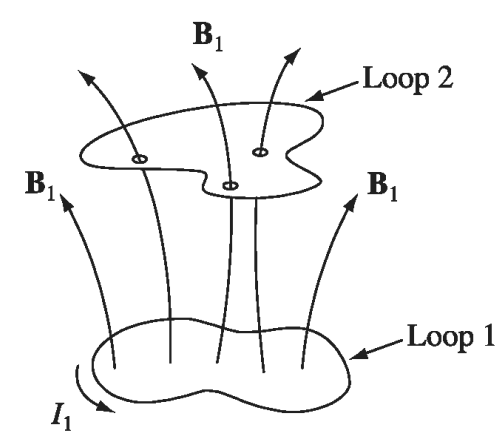
\includegraphics[width=0.5\textwidth]{inductance.png}
\end{center}
An emf $\E_2$ will be induced in Loop 2\footnote{
Technically, we can't use things like the Biot-Savart law and Ampere's law
exactly, since we developed those only for magnetostatics. We can use these
approximately in this case, since unless we're looking at very rapidly changing
fields, these equations are still appproximately accurate (the error is
negligible). We call this type of situation ``quasistatics.''}
Let's look at the chain of causation
that makes this happen. The $\E_2$ generated depends on the change in the flux
through Loop 2,
\[ \E_2 = -\pder{\Phi_B}{t} \]
The flux through Loop 2 depends on the strength of the magnetic field through
Loop 2:
\[ \Phi_2 = \iint\vec{B}_1\cdot\d\vec{a} \]
But the magnetic field $\vec{B}_1$ depends on the current $I_1$ in Loop 1:
\[ \vec{B}_1(\vec{r}) = \frac{\mu_0 I}{4\pi}
	\int \frac{\d\vec{\ell_1}\times\hat{\brcurs}}{\rcurs^2} \]
Based on this chain of causation, we can write
\begin{align*}
	\E_2 &= -\der{\Phi_B}{t}\\
	     &= -\der{\Phi_B}{I_1} \der{I_1}{t}\\
	     &= -M_{21} \der{I_1}{t}\\
	     &: M_{21} = \der{\Phi_B}{t}
\end{align*}
We call $M_{21}$ the mutual inductance of the two circuits. This value is based
on the circuits and their orientation relative to each other; if those two
remain constant, then
\[ \E = -M_{21}\der{I_1}{t} \]
If $M_{21}$ is constant, we can also say
\begin{align*}
	M_{21} &= \der{\Phi_2}{t}\\
	\d\Phi_2 &= M_{21} \d I_1\\
	\Phi_2 &= M_{21} I_1
\end{align*}
The units we use for the mutual inductance is the Henry (H). We can use the law
of Biot-Savart and the definition the vector potential to find the
\emph{Neumann formula}:
\[
	M_{21} = \oint_{C2}\oint_{C1}
		\frac{\d\vec{\ell}_1 \cdot \d\vec{\ell}_2}{\rcurs}
\]
This integral can be impossibly complicated if we're looking at anything other
than very simple geometry. The order of integration doesn't matter, implying
that the labels are basically arbitrary, so $M_{21} = M_{12} = M$. Since
the emfs are dependent on the mutual inductances, we can say that
\[ \E_1 = \E_2 \]
This is the basis for the transformer formula from PHY 151,
\[ \frac{\E_1}{E_2} = \frac{N_1}{N_2} \]
For a transformer, the flux in each circuit is boosted by increasing the number
of loops in that circuit. The emf ratio is adjusted by changing the loops in
each circuit.\\~\\
So far, we've looked at what happens in Loop 2 when we change the current in
Loop 1, but changing the current in Loop 1 also causes a change in the emf in
Loop 1. We can talk about the self-inductance, $L$:
\begin{align*}
	\E_1 &= -\der{\Phi_1}{t}\\
	     &= -\der{\Phi_1}{I_1}\der{I_1}{t}\\
	     &= -L\der{I_1}{t}\\
	     &: L = \der{\Phi_1}{I_1}
\end{align*}
This is the origin of Lenz's law: $\E$ opposes a change in flux. We could
re-derive a lot of equations, but realistically, whatever we said about $M$
also applies to $L$. If the geometry of Loop 1 is fixed, then
\begin{align*}
	\Phi_1 &= L I_1\\
	L &= \frac{\Phi_1}{I_1}
\end{align*}
We often just call $L$ the ``inductance.''

\begin{eg}
	A solenoid has $n$ turns per unit length, radius $R$, and carries a
	circuit $I$. Find $L$.\\
	\textbf{Solution.}
	From Chapter 5, we know the magnetic field for this solenoid,
	\[ B = \mu_0 n I \]
	Since the geometry is simple, we can talk about the flux
	\begin{align*}
		A &= \pi R^2\\
		\Phi &= BA\\
		     &= \mu_0 n I \pi R^2
	\end{align*}
	Which means the inductance is
	\[ L = \mu_0 n \pi R^2 \]
	If $n$ is very big, we will produce a huge emf, which we call a
	``back emf'' or ``choke.''
\end{eg}

\subsubsection{Energy in Magnetic Fields}
Establishing a current requires work (that is, it takes energy). The rate at
which we do work is called power:
\begin{align*}
	P = \der{W}{t} &= -\E I\\
		       &= -\left(-L\der{I}{t}\right)I\\
		       &= L\der{I}{t} I\\
	W &= \frac{1}{2}LI^2
\end{align*}
Given what we know about the flux, we can write
\begin{align*}
	\Phi &= LI\\
	     &= \iint_S \vec{B} \cdot \d\vec{a}\\
	     &= \oint_C \vec{A} \cdot \d\vec{\ell}\\
	W &= \frac{1}{2}LI^2\\
	  &= \frac{1}{2}\Phi I\\
	  &= \frac{1}{2}\left(\oint_C \vec{A} \cdot \d\vec{\ell}\right)\\
	  &= \frac{1}{2}\oint_C(\vec{A} \cdot \vec{I}) \d\ell
\end{align*}
We can generalize this to a volume current density $\vec{J}$ rather than
simply a current:
\[ W = \frac{1}{2}\oint_V (\vec{A} \cdot \vec{J}) \d\tau \]
Note that this is very similar to the equation for work we found in
electrostatics, but with the charge density replaced by the volume current
density.\\
From Ampere's law, we can take it a step farther:
\begin{align*}
	W &= \frac{1}{2\mu_0}\oint_V \vec{A} \cdot(\del \times \vec{B})\d\tau\\
	  &= \frac{1}{2\mu_0}\oint_V\left[
		\vec{B}\cdot(\del\times\vec{A}) -
		\del\cdot(\vec{A}\times\vec{B})\right]\d\tau
\end{align*}
By the divergence theorem of Gauss,
\[ W = \frac{1}{2\mu_0}\int_V B^2\d\tau -
	\frac{1}{2\mu_0}\int_S (\vec{A} \times \vec{B})\d\tau \]
If we have finite sources but integrate over all of space, the surface of $V$
is at infinity, so the second term disappears. This means that
\[ W = \frac{1}{2\mu_0} \int_{all\ space}B^2\d\tau \]

\subsection{Maxwell's Equations}
\subsubsection{The Displacement Current}
We've arrived at 4 quasistatic equations so far:
\begin{enumerate}
	\item Gauss's Law, based on observations and Coulomb's law:
		\[ \del \cdot \vec{E} = \frac{\rho}{\epsilon_0} \]
	\item The statement that there are no magnetic dipoles, based on
		observations and the Biot-Savart law:
		\[ \del \cdot \vec{B} = 0 \]
	\item Faraday's Law, based on observations:
		\[ \del \times \vec{E} = -\der{\vec{B}}{t} \]
	\item Ampere's Law, based on observations and the Biot-Savart law:
		\[ \del \times \vec{B} = \mu_0 \vec{J} \]
\end{enumerate}
Enter James Clark Maxwell, a math prodigy. In 1885, he sought to mathematically
sort out the observation-based physics of E\& M. Modern vector notation didn't
exist at the time, but he was still able to spot some inconsistencies.\\
Maxwell knew that $\del\cdot(\del\times\vec{V})=0$, but
\begin{align*}
	\del\cdot(\del\times\vec{B}) &= \del\cdot(\mu_0\vec{J})\\
	&= -\mu_0\epsilon_0\pder{(\del\cdot\vec{E})}{t} \neq 0
\end{align*}
Maxwell realized that in order to make this fit the vector equation we know,
he needed to add a term to Ampere's law:
\[ \del \times \vec{B} = \mu_0 \vec{J} + \mu_0 \epsilon_0 \pder{\vec{E}}{t} \]
With this change, all four equations are mathenatically consistent with each
other. Note that $\mu_0\epsilon_0 = 1.1\times10^{-17}$, so unless
$\pder{E}{t}$ is big enough to overwhelm $\sim10^{-17}$, this extra term would
be basically impossible to detect experimentally, especially at the time.
This extra term we added is called the \emph{displacement current}.

\subsubsection{Maxwell's Equations}
\begin{align*}
	\del \cdot \vec{E} &= \frac{\rho}{\epsilon_0} &
	\del \cdot \vec{B} &= 0\\
	\del \times \vec{E} &= -\pder{\vec{B}}{t} &
	\del \times \vec{B} &= \mu_0\vec{J} + \mu_0\epsilon_0\pder{\vec{E}}{t}
\end{align*}
Because all of the divergences and curls are known, as long as these are
finite, they satisfy the Helmholtz conditions, so we can know that we found
the only correct $\vec{B}$ and $\vec{E}$.\\
There's another way of writing these, that's mathematically equivalent, but
puts all the fields on the left, and the sources on the right, is
\begin{align*}
	\epsilon_0\del\cdot\vec{E} &= \rho &
	\del\cdot\vec{B} &= 0\\
	\del\times\vec{E} + \pder{\vec{B}}{t} &= 0 &
	\del\times\vec{B} - \mu_0\epsilon_0\pder{\vec{E}}{t} &= \mu_0\vec{J}
\end{align*}
What if we want to talk about what happens in materials? The only thing that
will change is those with a nonzero right-hand side. We already know Gauss's
law for materials,
\[ \vec{D} = \rho_f \]
So the only thing we need to fix is Ampere's law for materials. Recall from
Chapter 6 that we can write the current density as
\begin{align*}
	\vec{J} &= \vec{J}_f + \vec{J}_b\\
		&= \vec{J}_f + \del\times\vec{M}
\end{align*}
If we allow the formerly bound static charges to move, they will create a
current density that we call the polarization current density,
\begin{align*}
	\vec{J} &= \vec{J}_f + \vec{J}_b + \vec{J}_p\\
		&= \vec{J}_f + \del\times\vec{M} + \pder{\vec{P}}{t}
\end{align*}
Using this, we can re-write Ampere's Law:
\begin{align*}
	\del\times\vec{B} &=
	\mu_0\left(\vec{J}_f + \del\times\vec{M} + \pder{\vec{P}}{t}\right)
	+ \mu_0\epsilon_0 \pder{\vec{E}}{t}\\
	\del\times\frac{\vec{B}}{\mu_0} &= \vec{J}_f + \del\times\vec{M} +
		\pder{\vec{P}}{t} + \epsilon_0\pder{\vec{E}}{t}\\
	\del\times\left(\frac{\vec{B}}{\mu_0}-\vec{M}\right) &=
		\vec{J}_f + \pd{t}\left(\vec{P} + \epsilon_0\vec{E}\right)\\
	\del\times\vec{H} &= \vec{J}_f + \pder{\vec{D}}{t}
\end{align*}
This is where the term ``displacement current'' comes from---it's a current
due to the displacement $\vec{D}$.\\
So the full set of Ampere's equations for materials is
\begin{align*}
	\del \cdot \vec{D} &= \rho_f &
	\del \cdot \vec{B} &= 0\\
	\del \times \vec{E} + \pder{\vec{B}}{t} &= 0 &
	\del \times \vec{H} &= \vec{J}_f + \pder{\vec{D}}{t}
\end{align*}
But Maxwell didn't stop there! He knew that he could take the curl of a curl:
\[ \del\times(\del\times\vec{E}) = -\pd{t}(\del\times\vec{B}) \]
Using the vector identity, the LHS in a vacuum turns into
\begin{align*}
	\del\times(\del\times\vec{E})&=\del(\del\cdot\vec{E})-\nabla^2\vec{E}\\
				     &=-\nabla^2\vec{E}
\end{align*}
The right-hand side becomes
\begin{align*}
	-\pd{t}\left(\pd{t}\del\times\vec{B}\right) &=
		-\pd{t}\left(\mu_0\epsilon_0\pder{\vec{E}}{t}\right)\\
		&= -\mu_0\epsilon_0\pder{^2\vec{E}}{t^2}
\end{align*}
Together,
\[ \nabla^2\vec{E} = \mu_0\epsilon_0\pder{^2\vec{E}}{t^2} \]
This is a wave equation for $\vec{E}$! We can do the same thing for $\vec{B}$:
\begin{align*}
	\del\times(\del\times\vec{B})&=\mu_0\epsilon_0\pd{t}\del\times\vec{E}\\
	\del(\del\cdot\vec{B})-\nabla^2\vec{B}&=
		\pd{t}\left(-\mu_0\epsilon_0\pder{\vec{B}}{t}\right)\\
	\nabla^2\vec{B}&=
		\mu_0\epsilon_0\pder{^2\vec{B}}{t^2}\\
\end{align*}
This is also a wave equation, but for $\vec{B}$ now! Notice how similar they
are.\\
These waves propagate through the vacuum with speed
\[ v = (\epsilon_0\mu_0)^{1/2} = 3\times10^8 \mathrm{m/s} \]
The speed of light! A quote from Maxwell:
``Light consists of transverse undulations of the same medium which is the
cause of the electric and magnetic phenomena.''

\end{document}
